\documentclass[11pt]{article}

%==============Packages & Commands==============
\usepackage{graphicx}
\usepackage{fancyvrb}
\usepackage{tikz}
%%%<
\usepackage{verbatim}
%\usepackage[active,tightpage]{preview}
%\PreviewEnvironment{tikzpicture}
%\setlength\PreviewBorder{5pt}%

\usepackage{geometry}                		% See geometry.pdf to learn the layout options. There are lots.
% \geometry{a4paper}                   		% ... or a4paper or a5paper or ...
%\geometry{landscape}                		% Activat\usetikzlibrary{arrows}e for for rotated page geometry
%\usepackage[parfill]{parskip}    		% Activate to begin paragraphs with an empty line rather than an indent
\usepackage{graphicx}				% Use pdf, png, jpg, or eps§ with pdflatex; use eps in DVI mode
								% TeX will automatically convert eps --> pdf in pdflatex
\usepackage{amssymb}

\usepackage[ruled,vlined]{algorithm2e}
\usetikzlibrary{arrows}
\usepackage{alltt}
\usepackage[T1]{fontenc}
\usepackage[utf8]{inputenc}
\usepackage{indentfirst}
\usepackage[longnamesfirst]{natbib} % For references
\bibpunct{(}{)}{;}{a}{}{,} % Reference punctuation
\usepackage{changepage}
\usepackage{setspace}
\usepackage{booktabs} % For tables
\usepackage{rotating} % For sideways tables/figures
\usepackage{amsmath}
\usepackage{multirow}
\usepackage{color}
\usepackage{dcolumn}
\usepackage{comment}
\usepackage{xcolor, colortbl}
%\usepackage{fullwidth}
\newcolumntype{d}[1]{D{.}{\cdot}{#1}}
\newcolumntype{.}{D{.}{.}{-1}}
\newcolumntype{3}{D{.}{.}{3}}
\newcolumntype{4}{D{.}{.}{4}}
\newcolumntype{5}{D{.}{.}{5}}
\usepackage{float}
\usepackage[hyphens]{url}
%\usepackage[margin = 1.25in]{geometry}
%\usepackage[nolists,figuresfirst]{endfloat} % Figures and tables at the end
\usepackage{subfig}
\captionsetup[subfloat]{position = top, font = normalsize} % For sub-figure captions
\usepackage{fancyhdr}
%\makeatletter
%\def\url@leostyle{%
%  \@ifundefined{selectfont}{\def\UrlFont{\sf}}{\def\UrlFont{\small\ttfamily}}}
%\makeatother
%% Now actually use the newly defined style.
\urlstyle{same}
\usepackage{times}

\usepackage{lscape}
% \usepackage{mathptmx}
%\usepackage[colorlinks = true,
%						bookmarksopen = true,
%						pagebackref = true,
%						linkcolor = black,
%						citecolor = black,
% 					urlcolor = black]{hyperref}
%\usepackage[all]{hypcap}
%\urlstyle{same}
\newcommand{\fnote}[1]{\footnote{\normalsize{#1}}} % 12 pt, double spaced footnotes
\def\citeapos#1{\citeauthor{#1}'s (\citeyear{#1})}
\def\citeaposs#1{\citeauthor{#1}' (\citeyear{#1})}
\newcommand{\bm}[1]{\boldsymbol{#1}} %makes bold math symbols easier
\newcommand{\R}{\textsf{R}\space} %R in textsf font
\newcommand{\netinf}{\texttt{NetInf}\space} %R in textsf font
\newcommand{\iid}{i.i.d} %shorthand for iid
\newcommand{\cites}{{\bf \textcolor{red}{CITES}}} %shorthand for iid
%\usepackage[compact]{titlesec}
%\titlespacing{\section}{0pt}{*0}{*0}
%\titlespacing{\subsection}{0pt}{*0}{*0}
%\titlespacing{\subsubsection}{0pt}{*0}{*0}
%\setlength{\parskip}{0pt}
%\setlength{\parsep}{0pt}
%\setlength{\bibsep}{2pt}
%\renewcommand{\headrulewidth}{0pt}

%\renewcommand{\figureplace}{ % This places [Insert Table X here] and [Insert Figure Y here] in the text
%\begin{center}
%[Insert \figurename~\thepostfig\ here]
%\end{center}}
%\renewcommand{\tableplace}{%
%\begin{center}
%[Insert \tablename~\theposttbl\ here]
%\end{center}}

\newcommand\independent{\protect\mathpalette{\protect\independenT}{\perp}}
\def\independenT#1#2{\mathrel{\rlap{$#1#2$}\mkern2mu{#1#2}}}
\newcommand{\N}{\mathcal{N}}
\newcommand{\Y}{\bm{\mathcal{Y}}}
\newcommand{\bZ}{\bm{Z}}

\usepackage[colorlinks = TRUE, urlcolor = black, linkcolor = black, citecolor = black, pdfstartview = FitV]{hyperref}


%============Article Title, Authors==================
\title{\vspace{-2cm} Government websites as data: A methodological pipeline for collection, processing, and text analysis }


\author{ Markus Neumann \and Fridolin Linder \and Bruce Desmarais} \date{\today}



%===================Startup=======================
\begin{document}
\maketitle



%=============Abstract & Keywords==================

\begin{abstract}

A local government's website is a standard and general source of information for citizens and other community stakeholders. Accordingly, government websites have become prominent sources of data for a variety of research agendas in public administration, public policy, and political science. Existing research has relied on manual methods of website data collection and processing. Reliance on manual collection and processing limits the scale and scope of website content analysis.  We develop a methodological pipeline that researchers can follow in order to gather, process, and analyze website content with established text analysis techniques. First, for the acquisition of website data, we cover approaches to automated scraping methods. Second, pre-processing is a particularly vital step in text analysis, but when websites are concerned, additional measures need to be taken in order to guard against potential sources of bias. We propose a new method for dealing with the kind of duplicated content that is commonly found in government websites. Finally, we illustrate methods of text analysis using automatically gathered and pre-processed website content. We illustrate our methodological pipeline through a new and innovative dataset---the websites of municipal governments in Indiana and Louisiana. We build upon recent research that analyzes how change and variation in the partisan control of government relates to content made available on the government's website. We explore the association between mayoral partisanship and the content of city websites.
%\noindent We explore the effect of transitions of power in municipal governments on the content of their websites. We hypothesize that when party control changes, city administrators modify the contents of their websites in order to fit the agenda of the new incumbent. To test this theory, we study cities in Indiana and Louisiana, two states in which all municipal elections are partisan and the parties of the candidates appear on the ballots. Snapshots of websites before and after transitions of power are acquired through the Wayback Machine. We apply statistical topic models based in latent dirichlet allocation, focusing on changes to the websites. We present results on both which topics see the greatest degree of change associated with transitions in city administrations, and how the topics modified differ with regard to political parties.

\end{abstract}
\thispagestyle{empty}
% \doublespacing
% Description of the possible challenges
\section{Introduction}

Local governments convey voluminous information about all aspects of their policymaking, policy implementation, and public deliberation, via their official websites. The vital role of official websites in connecting the government and the governed has motivated a wave of research on the contents of government websites \citep[e.g., ][]{grimmelikhuijsen2010transparency,wang2005evaluating,osman2014cobra}. Despite the potential for automated scraping of website contents, the conventional approach to data collection in projects focused on government websites involves manual content extraction from each website in the dataset. Though highly accurate, the manual approach to data collection is costly, and cannot be scaled to capture even a fraction of the volume of content available on government websites. In this paper we present a methodological pipeline that can be used to automatically scrape government websites in order to build datasets that can be used for text analysis. We provide an illustrative application in which we explore the ways in which the textual contents on city government websites in Indiana and Louisiana correlate with the partisanship of the city mayor.

Though there exists a variety of software tools that are designed to automatically scrape all of the files available at a website \citep{glez2013web}, raw website downloads have to be processed significantly before the files are adequately prepared for text analysis. We describe and provide solutions to two central challenges in automatically gathering and analyzing website textual contents. First, plain text must be extracted from the files. This involves purging the files of syntax in HTML and other programming languages, and discarding any other character encoding errors that result from reading the files. This challenge would arise in any context in which researchers sought to study the textual contents of websites, and is not unique to comparative analysis of government websites. The second challenge we address in our methodological pipeline is, however, specific to the research objective of comparing websites on the basis of a common lexicon. For any two governments, the textual signatures that most dramatically differentiate the textual contents of their websites consist of what we can call ``boilerplate'' text---header, footer, or other titling text that is designed to identify the website as being associated with a specific government entity (e.g., ``Welcome to the city of Santa Cruz'', ``The City of Los Angeles welcomes you''). This boilerplate text is replicated across many files that are associated with a government's website, but it provides little information regarding the form and/or function of the government. The second methodological innovation we offer in our pipeline is designed to minimize the impact of this boilerplate text on the comparative analysis of government website content. 

Government websites provide information about how public policies shape the lives of local residents, and how local residents can engage with government to shape public policy. As such, government websites reflect both the results of, and inputs to, the political leadership in the city. In our illustrative application we explore the ways in which the contents of city government websites differ on the basis of the partisanship of the city's elected executive. A substantial body of research has found that the partisanship of the mayor affects city governance along multiple dimensions, including city budget priorities \citep{de2016mayoral}, policies affecting inequality in cities \citep{einstein2016mayors}, and framing of criminal justice policy \citep{marion2013mayor}. Furthermore, recent media coverage of changes to government websites that follow transitions in party control suggest that changes in web content are salient government actions, as perceived by the general public \citep{sharfstein2017science,kirby2017trump,duarte2017deniable} . We study whether significant differences between city governments based on mayoral partisanship are reflected in the contents of city websites.


\section{The Significance of Government Website Content}
% \cite{grimmelikhuijsen2012developing} conduct an enormously relevant study. Insofar as we analyze what predicts openness of government websites, we will be replicating and building upon this study. They focus on Dutch municipal websites, and their approach is fairly limited in scope and highly manual (which we can compliment). For example, one of the dependent variables ``Decision-making transparency,'' is measured ``using a discrete (1/0) indicator for whether the underlying principles or reasons for local air pollution policies were given on the Web site.'' 

 According to \cite{Mayhew1974}, politicians engage in advertising, credit claiming and position taking in order to get re-elected. Official city websites allow mayors to do all three. Their offices frequently take a prominent position on the frontpage, and many websites also feature a picture of the candidate. In local politics, where campaign funds are low, this lends the incumbent a crucial advantage in becoming more well-known among her constituents. Furthermore, municipal politics gives incumbents clear and tangible achievements they can point to, such as completed infrastructure projects, the acquisition of federal or state funding, or the hosting of city-wide events. City websites present an opportunity for local officials to brandish these accomplishments. Finally, they also give mayors a platform from which they can advertise their political beliefs. On municipal websites, this may not manifest in the form of brazen partisanship, but more subtle avenues are available. As noted by \cite{einstein2016mayors}, there are stark differences in the spending preferences of Democratic and Republican mayors. City websites can then be used to communicate the stance of a mayor on social or economic programs. Another advantage of websites with regard to communication is that unlike direct social interactions, officials have full control over them.

Some papers on how government websites are used
\begin{itemize}
\item \cite{sandoval2012government}, p.S74, ``Usually citizens access government websites to find information and
data for decision making''.
\item In a survey conducted among a random sample of citizens in the state of Georgia in 2000, \cite{thomas2003new} found that nearly 25\% of internet users in the sample reported visiting a local government website in the previous twelve months to gather information. We would expect that number to be even larger nearly two decades later.
\item \cite{tolbert2006effects} p. 355, ``We ?nd that users of local government Web sites are more likely to trust local governments, controlling for other demo-graphic factors, and that the use of government Web sites is associated with other positive attitudes, espe-cially for federal and local governments. ''
\end{itemize}


In addition to the use of city websites for the politicians that control them, variance in content also matters  with regard to the people who visit them. Local residents likely rely on city websites to get news about events, hot-button political issues specific to their city, contact city officials or find out addresses or opening hours of city institutions. Visitors use city websites to look up local attractions, which are often described in great detail. Similarly, prospective residents looking to move, might rely on city websites to inform their decision on whether to relocate there. An inviting website emphasizing the city's receptiveness to new residents might make a real difference here. Finally, city websites frequently feature sections on business, but there is a lot of variance in this area: Some emphasize economic development, properties, or transportation, whereas others focus on undeveloped land and other business opportunities. Differences in websites likely say something about a city's economic profile, with potential repercussions for the political realm.

The literature making use of scraped websites clusters into a number of categories. One, and most pertinent to our own endeavors, the e-governance literature which discusses the online presence of governments from a usability and public service point of view. For the most part, research in this category develops a classification scheme to rate websites in terms of accessibility, ease-of-use and function, and then hand-codes a set of websites according to these criteria \citep{Urban2002,Armstrong2011,Feeney2017}. As an example, \cite{grimmelikhuijsen2012developing} study local government websites with the goal of uncovering how they aid the goal of transparency. To this end, they analyze a set of Dutch municipalities in which air quality had deteriorated. The authors test whether local governments provide citizens with information about potential complications and solutions associated with this issue. Like most e-government studies however, this publication does not make any use of automated text analysis.

Websites have also played a major role in the field of media studies, as scholars have scraped and analyzed the online presence of newspapers, as well as the more diffuse world of online political blogs \citep{Adamic2005,Gentzkow2010}. \cite{Lin2011} provide a good example for a study which makes extensive use of automated content analysis - a necessity arising from its dataset of 66830 blog posts and 57221 online news articles. The authors estimate the political slant of these entities by counting the frequencies with which politicians of either side are mentioned and determine that blogs are generally more biased. Unfortunately for us, the authors don't go into the details of their text analysis, and offer no information on the acquisition and pre-processing of the data.

Another well-known example fitting into this area of study is the set of studies conducted by King et al. \citep{KING2013,King2014,KING2017}, in which the authors study censorship by the country's government on its lively blogosphere. However, the authors also provide no information on how their data was collected ``our extensive engineering effort, which we do not detail here for obvious reasons [...]''.

The websites of politicians and their parties have also fallen under scholarly scrutiny. Researchers have found that in order to identify the constituencies, motives and modes of communication of these actors, their websites can be very illuminating sources of information \citep{Druckman2009,Druckman2010,Cryer2017,Esterling2011,Esterling2011a,Norris2003,Therriault2010}. \cite{Druckman2009,Druckman2010} rely on the Mational Journal to find the websites, then hand-coded them. \cite{Cryer2017} provides fairly little information, but does mention the fact that she relied on Archive-it, the webservice of the Internet Archive we discussed recently. \cite{Esterling2011,Esterling2011a} rely on hand-coded data by the Congressional Management Foundation, a nonprofit organization which aims to assist Congress. \cite{Therriault2010} (a working paper) actually portends to use automated text analysis, and also has the most extensive overview of the associated methodology. However, the division of the website into sections (home page, topics, issues, details) is done by hand, and the actual analysis is incomplete. The author acquired the websites from the Library of Congress (which only collected them from legislators who actually consented, and Therriault notes that this causes nonrandom missingness).

Importantly for us, research analyzing and improving the scraping, pre-processing and analysis methods of this literature is scarce. \cite{Eschenfelder2002} provide something of an overview of how how federal websites should be assessed from an e-governance point of view, but they largely focus on the substantive criteria that should be fulfilled, rather than the technical aspects of website acquisition and analysis.




\section{Data}
In this section we introduce the data we use in our application---the analysis of municipal websites in Louisiana and Indiana. The General Services Administration (GSA) maintains all .gov addresses, and provides a complete\footnote{Domains used for testing and internal programs are excluded.} list of all such domains to the public through GitHub\footnote{https://github.com/GSA/data/tree/gh-pages/dotgov-domains}. This list is updated once per month - we rely on the version released on January 16, 2017. The data from the GSA contains the following variables: One, domain name, specifically, the all-uppercase version of domain and top-level domain (for example, 'ABERDEENMD.GOV'). Two, the type of government entity to which the domain is registered, such as city, county, federal agency, etc. Three, for federal agencies, the name is specfied. Finally, the city in which the domain is registered, is noted.

Here, we focus only on cities. As a first step, we use a webdriver-controlled browser (Firefox/Selenium/Geckodriver) to test whether all of the city websites actually work. Of the 2425 domains listed by the GSA as cities, 292 are not accessible. Furthermore, the .gov domain, as registered at the GSA, is frequently not the website a city actually uses. In many cases, these sites redirect to another address, sometimes not a .gov domain (in this case, we simply use this domain). We record these URLs.

In order to provide an overview of our coverage (as not all cities, towns and villages use .gov addresses), we merge this list with U.S. Census data\footnote{http://www2.census.gov/programs-surveys/popest/datasets/2010-2015/cities/totals/sub-est2015\_all.csv}. Here, several limitations in the GSA data need to be accounted for: One, even though the GSA nominally separates websites of cities and counties, some of the domains categorized as cities actually belong to counties. The same is true for townships and boroughs. Ergo, we eliminate all websites belonging to these three types of entities by hand. Furthermore, the city name, as given by the GSA, refers to the city in which the domain is registered, which is not necessarily equivalent to the city the website serves. In many cases, a website of a larger city may be registered to one of its subdivisions (for example, the website of New York is registered to Brooklyn), or vice versa (for example, the website of Homecroftin, a small town within Indianapolis, is registered to the city as a whole). Consequently we fix mismatches between websites and cities manually. Finally, a number of cities are simply misspelled, which we also correct by hand.

% latex table generated in R 3.4.0 by xtable 1.8-2 package
% Tue May 23 19:28:26 2017
\begin{table}[ht]
	\centering
	\begin{tabular}{lrrr}
		\hline
		Filetype & current & before & after \\
		\hline
		& 51455 & 13866 & 19199 \\
		pdf & 9646 & 5489 & 7544 \\
		jpg & 5216 & 1988 & 3512 \\
		html & 3767 & 17842 & 17596 \\
		aspx & 2832 & 4356 & 3271 \\
		png & 2714 & 2327 & 3684 \\
		gif & 1068 & 664 & 1077 \\
		JPG & 478 & 182 & 263 \\
		1 & 443 &  61 &  54 \\
		css & 390 & 265 & 518 \\
		js & 350 & 255 & 468 \\
		htm & 264 & 295 & 256 \\
		docx & 203 & 106 & 120 \\
		doc & 167 &  70 & 130 \\
		asp & 161 & 201 & 211 \\
		svg &  87 &  55 &  69 \\
		php &  83 & 157 & 241 \\
		\hline
	\end{tabular}
	\caption{The most common file types in scraped websites}
\end{table}


\begin{landscape}
% latex table generated in R 3.4.0 by xtable 1.8-2 package
% Tue May 23 19:35:22 2017
\begin{table}[ht]
	\centering
	\footnotesize
	\begin{tabular}{lrrrrrrrrr}
		\hline
		Website & current\_size & current\_files & before\_size & before\_files & after\_size & after\_files & size\_change & files\_change & control\_change \\
		\hline
		attica-in.gov & 61988 & 1417 & 7528 & 164 & 55956 & 1390 & 7.43 & 8.48 & 0.00 \\
		bedford.in.us & 57628 & 560 & 27452 & 182 & 46388 & 525 & 1.69 & 2.88 & 0.00 \\
		cityofboonvilleindiana.com & 9848 & 110 & 16996 & 172 & 20784 & 229 & 1.22 & 1.33 & 0.00 \\
		frankfort-in.gov & 205368 & 2652 & 12208 & 242 & 138360 & 1077 & 11.33 & 4.45 & 0.00 \\
		warsaw.in.gov & 298440 & 2117 & 26844 & 539 & 360400 & 2036 & 13.43 & 3.78 & 0.00 \\
		www.bloomington.in.gov & 131128 & 2713 & 443360 & 14384 & 247096 & 9640 & 0.56 & 0.67 & 0.00 \\
		www.brazil.in.gov & 43056 & 845 & 34472 & 625 & 55152 & 1214 & 1.60 & 1.94 & 0.00 \\
		www.carmel.in.gov & 2270016 & 8727 & 1919344 & 5361 & 899900 & 2219 & 0.47 & 0.41 & 0.00 \\
		www.ci.auburn.in.us & 183296 & 1025 & 21444 & 345 & 23564 & 211 & 1.10 & 0.61 & 0.00 \\
		www.cityoffortwayne.org & 2136424 & 4378 & 266784 & 3582 & 233600 & 3018 & 0.88 & 0.84 & 0.00 \\
		www.cityofhobart.org & 722000 & 2463 & 44192 & 650 & 62660 & 1037 & 1.42 & 1.60 & 0.00 \\
		www.evansvillegov.org & 6345932 & 11844 & 290784 & 1281 & 1697224 & 6853 & 5.84 & 5.35 & 0.00 \\
		www.gary.in.us & 373888 & 1227 & 121812 & 485 & 157140 & 719 & 1.29 & 1.48 & 0.00 \\
		www.huntingburg-in.gov & 388680 & 2496 & 8644 & 213 & 375900 & 1953 & 43.49 & 9.17 & 0.00 \\
		www.jasperindiana.gov & 561968 & 4013 & 55900 & 460 & 439072 & 2224 & 7.85 & 4.83 & 0.00 \\
		www.lakestation-in.gov &  48 &   2 & 7724 &  84 & 257272 & 1097 & 33.31 & 13.06 & 0.00 \\
		www.linton-in.gov &  32 &   1 &  24 &   2 &  24 &   2 & 1.00 & 1.00 & 0.00 \\
		www.madison-in.gov & 531044 & 1848 & 36636 & 575 & 191624 & 1444 & 5.23 & 2.51 & 0.00 \\
		www.martinsville.in.gov & 46792 & 1463 & 71628 & 1052 & 80944 & 800 & 1.13 & 0.76 & 0.00 \\
		www.monticelloin.gov & 33656 & 753 & 18120 & 448 & 100680 & 2104 & 5.56 & 4.70 & 0.00 \\
		www.newhavenin.org & 84364 & 626 & 2524 &  86 & 6792 & 334 & 2.69 & 3.88 & 0.00 \\
		www.richmondindiana.gov & 250968 & 1042 & 217252 & 918 & 401672 & 2422 & 1.85 & 2.64 & 0.00 \\
		www.southbendin.gov & 1264076 & 4749 & 454456 & 3286 & 1424136 & 2562 & 3.13 & 0.78 & 0.00 \\
		connersvillecommunity.com & 170688 & 569 & 162316 & 815 & 187276 & 808 & 1.15 & 0.99 & 1.00 \\
		www.batesvilleindiana.us & 166564 & 2348 & 39592 & 496 & 95696 & 1310 & 2.42 & 2.64 & 1.00 \\
		www.cityofrisingsun.com & 994956 & 3311 & 321400 & 1268 & 80848 & 868 & 0.25 & 0.68 & 1.00 \\
		www.cityofrockport-in.gov & 12068 &  98 & 5148 &  16 & 12068 &  98 & 2.34 & 6.12 & 1.00 \\
		www.elkhartindiana.org & 1132828 & 2345 & 5588 & 123 & 6204 & 223 & 1.11 & 1.81 & 1.00 \\
		www.elwoodcity-in.org & 224412 & 765 & 5000 & 123 & 139692 & 517 & 27.94 & 4.20 & 1.00 \\
		www.indy.gov & 5726048 & 9675 & 6119260 & 10451 & 4984080 & 7981 & 0.81 & 0.76 & 1.00 \\
		www.northvernon-in.gov & 272016 & 403 & 3132 & 112 & 289336 & 416 & 92.38 & 3.71 & 1.00 \\
		www.winchester-in.gov & 364592 & 2480 & 6508 & 135 & 45488 & 567 & 6.99 & 4.20 & 1.00 \\
		\hline
	\end{tabular}
	\caption{Number of files and size of websites}
\end{table}

\end{landscape}

For some cities, whose websites make heavy use of JavaScript, this method does not lead to satisfying results. Consequently we restricted our corpus to cities with at least 3 documents.


\section{The Web to Text Pipeline}

In the methodological pipeline from native website files to text data that is appropriate for comparative analysis we address two methodological challenges. First, though they contain significant amounts of text, websites are not comprised of clean plain text files. Rather, the files available at websites are of multiple types, including HTML, PDF, word processor, plain text, and image files. The first step in the methodological pipeline is aimed simply at extracting clean plain text from this heterogeneous file base. The second step in our methodological pipeline is to process the text to remove boilerplate language---language that is effective at differentiating one website from another, but is uninformative regarding policy or process differences between governments. We describe these methodological steps in this section.

\subsection{Site to Text Conversion}
For the most part, the file type of a document can be correctly determined through its ending. However, there are exceptions to this, which, if ignored, can lead to large amounts of garbage text, stemming from incorrectly converted documents, as well as a general decrease in the amount of usable data. Two issues in particular need to be addressed: One, HTML files on city websites frequently do not have an ending, but are still perfectly readable if correctly identified as such. Second, some documents contain the incorrect file ending - for example, we found thousands of documents on the New Orleans city website that ended in .html, when they were actually PDFs. To accurately assess their type, we read in the first line of each document, which, if it is an HTML or PDF file, contains a string indicating as much. Consequently we rename all documents so that their file ending reflects their actual file type. This is strictly necessary, because we rely on the readText R package\footnote{We have also experimented with several Unix-based alternatives, but found that they largely led to the same results.} - which determines a document's type solely through its ending - to convert the files to plain text.

The text documents are then read into R line by line, converted to UTF-8 and then stripped of dates, punctuation, numbers and words connected by underscores. At this point, the documents of one city still closely resemble one another in the form of boilerplate content, be it website elements (i.e. "You are here", "Home", "Directory" etc.) in html documents, or commonly used forms or phrases in pdfs, doc and docx files. This is an issue, because it clusters documents around the cities from which they originate in a way that has nothing to do with their actual content. In other words, the signal would be drowned out by the noise. Our solution to this problem is described in more detail in section \ref{boilerplate}.
Preprocessing further includes setting every character to lowercase, as well as the removal of bullet points which frequently occur in html documents, extraneous whitespace, xml documents mislabeled as html files, and empty documents. Furthermore, some documents contain gibberish, often as a result of faulty or impartial OCR. To combat this problem, we employ two solutions. One, we use spellchecking, implemented through the hunspell R package, to remove all non-English words.\footnote{Some of the cities, for example Los Angeles, do contain a sizable proportion of Spanish content. The analysis of this content is beyond the scope of this paper, but could be explored in future work, for example relying on multilingual word embeddings. Since the removal of non-English words is very computationally-intensive, we only take this step at the end of the preprocessing process, the result of which might be a slightly adverse effect on the accuracy of the boilerplate classifier.} However, hunspell does not cover everything, either because some tokens are not actual words (for example artifacts from defective encoding), or because random sequences of characters just so happen to form words that exist in a dictionary (for example "eh" or "duh"). Since we rely on a bag-of-words model in which syntax does not matter, we can ameliorate these problems by removing all text except for whitespaces and the characters that appear in the English alphabet. Since a lot of the nonsensical text tends to be quite repetitive, we also delete all documents in which the proportion of unique to total number of tokens is less than 0.15. Furthermore, hunspell does not spellcheck individual characters or two-character words, so we remove these token types entirely (none of these words are of any substantive relevance to our research question). Since these pre-processing steps reduce documents which are largely unsuitable to only a few words of texts that don't make much sense, we also remove all remaining documents containing less than 50 tokens. Finally, to remove words that are extremely rare (which also has the advantage of eliminating any remaining oddities) and thus add nothing substantive to our models while increasing their computational cost, we also discard any token types that occur in only one document.

\subsection{Boilerplate Removal}\label{boilerplate}
As noted above, city websites contain a large amount of text that is uninformative for its actual content and therefore a hindrance to correct analysis by automatic text processing methods. This is a common issue with textual data in which informative content is embedded in technically structured documents. See, e.g., \citet{burgess2016legislative,wilkerson2015tracing} and \citet{linder2018text} for examples of boilerplate removal in the analysis of legislative text. Consequently we remove this content as following: Each line of every document is compared to every line in every other document belonging to the same city. We count how many times each line is duplicated for that city. We remove any line occuring more than our chosen threshold of 10.\footnote{Empirically, lines tend to be duplicated either hundreds of times, or only once or twice, if at all.} This means that each document only retains the information that is particular about it. We implement this algorithm through hash tables, which reduces the computational complexity from O($N^2$) to O($N$). Before this step is taken, we remove numbers and dates from the documents because they frequently make lines unique, despite the fact that they are virtually the same (for example different days on a city calendar).

\subsection*{Boilerplate Classification}

In order to determine whether a line should be discarded, we train a simple classifier. We sampled 100 lines from documents from Anchorage, Alaska - 20 of which ocurred 1-4, 5-9, 10-19, 20-39 and over 40 times within the city\footnote{For the paper, we should increase the sample size sample lines from more than just one city. But I don't want to go through the effort of doing all this hand-coding until we're actually sure if and how we are going to use this.}. These lines were hand-coded as either substantively useful or useless. Then we trained a logit model with this usefulness measure as the dependent variable. The independent variables were: (1) number of times the line was duplicated within the city, (2) length of the line, in characters, (3) number of tokens in the line, and (4) the average keyness of the terms in the line. The purpose of these covariates is as following:

The length of the line and the number of tokens are a way to find lines consisting of only a word or two. This is highly predictive of lines which are used as website headers and navigational elements, which are of of zero substantive interest to us. These terms also happen to be fairly common, which causes them to be overweighted by the topic model.

To directly address the latter problem, a measure for the number of times a line is duplicated within a city is included. Many lines occur hundreds or even thousands of times on a single website, and therefore are terms that are highly predictive of the website, which causes the topic model to create topics that are highly correlated with cities.

Finally, the keyness measure: This indicator shows whether a term occurs disproportionally frequently in one document collection, compared to another. In our case, this would be one city's documents, compared to all others. Mathematically, this is a simple chi-square test, asserting whether the frequency of a word in a city is greater than its expected count, as determined by its count in all other documents, and the number of tokens in the city. The variable used in the model is the chi-square value of this test for each word (which varies and is therefore calculated individually for each city).\footnote{Or alternatively, the log of the absolute chi-square value, after which the previously negative values are made negative again.}

A regression table for this model can be found in table 3. The associated accuracy in 5-fold cross-validation is 0.8325. The cross-validation accuracy of a simplified model with only the number of characters as a covariate is 0.825 (table 4). A model with the four covariates described above as well as interaction terms between each of them yields an accuracy of 0.885 (table 5).


% Table created by stargazer v.5.2 by Marek Hlavac, Harvard University. E-mail: hlavac at fas.harvard.edu
% Date and time: Wed, May 23, 2018 - 03:39:09 PM
\begin{table}[!htbp] \centering 
  \caption{} 
  \label{} 
\begin{tabular}{@{\extracolsep{5pt}}lc} 
\\[-1.8ex]\hline 
\hline \\[-1.8ex] 
 & \multicolumn{1}{c}{\textit{Dependent variable:}} \\ 
\cline{2-2} 
\\[-1.8ex] & class \\ 
\hline \\[-1.8ex] 
 nchars & $-$0.003 \\ 
  & (0.002) \\ 
  & \\ 
 nwords & $-$0.018 \\ 
  & (0.013) \\ 
  & \\ 
 medianDocMidDist & 0.056 \\ 
  & (0.158) \\ 
  & \\ 
 prob & 8.515$^{**}$ \\ 
  & (3.856) \\ 
  & \\ 
 freq & $-$0.00000 \\ 
  & (0.00000) \\ 
  & \\ 
 Constant & 0.813$^{***}$ \\ 
  & (0.048) \\ 
  & \\ 
\hline \\[-1.8ex] 
Percent Correctly Predicted & 0.844 \\ 
Precision & 0.795 \\ 
Recall & 0.978 \\ 
F1-Score & 0.876 \\ 
Observations & 400 \\ 
Log Likelihood & $-$193.686 \\ 
Akaike Inf. Crit. & 399.372 \\ 
\hline 
\hline \\[-1.8ex] 
\textit{Note:}  & \multicolumn{1}{r}{$^{*}$p$<$0.1; $^{**}$p$<$0.05; $^{***}$p$<$0.01} \\ 
\end{tabular} 
\end{table} 

% latex table generated in R 3.4.4 by xtable 1.8-2 package
% Sat Jul 28 20:34:44 2018
\begin{table}[ht]
\centering
\begin{tabular}{rr}
  \hline
 & Value \\ 
  \hline
Percent Correctly Predicted & 0.87 \\ 
  Precision & 0.87 \\ 
  Recall & 0.91 \\ 
  F1-Score & 0.89 \\ 
   \hline
\end{tabular}
\caption{Performance metrics for random forest boilerplate classifier, with inverse probability weights.} 
\label{randomForest}
\end{table}


% latex table generated in R 3.4.4 by xtable 1.8-2 package
% Sat Jul 28 20:34:45 2018
\begin{table}[ht]
\centering
\begin{tabular}{lr}
  \hline
Feature & Importance \\ 
  \hline
nchars & 100.00 \\ 
  nwords & 83.70 \\ 
  medianDocMidDist & 13.50 \\ 
  freq & 0.00 \\ 
   \hline
\end{tabular}
\caption{Variable importance for random forest boilerplate classifier, with IPW weighting.} 
\label{randomForestVarimp}
\end{table}



Although not implemented yet, the idea is to use this classifier to flag and remove all lines that are not classified as substantively useful (if we want to be cautious, we could choose to only do that for lines that are classified as, for example, having a 60\% chance (or some other number greater than 50\%) of not being substantively useful).

\section{Bag-of-Words Text Analysis}

We illustrate the analysis of municipal website content using bag-of-words (BoW) methods. BoW methods are methods of text analysis that do not take into account the sequence or placement of words in text---just the presence and frequency of words. 


\subsection{Informative Dirichlet model}
%However, \cite{Monroe2008} advise against using these types of methods in this context because they get the data generation process backwards: Our theory assumes that party leads to variation in writing, and yet we rely on the documents to predict party, in spite of the fact that we actually have perfect knowledge of it.

For the analysis of the data, we present two approaches, the first being the informative dirichlet model developed by \citep{Monroe2008}. This approach aims to account for the fact that some words naturally occur more than others by applying a Dirichlet prior based on the distribution of words in random text. Table \ref{tabFightinIN} shows the top words for both Democrats and Republicans - and accomplishes, to some extent, the goal of \citep{Monroe2008} of banishing frequent words from this list and supplanting them with text with greater semantic, and in our case, partisan meaning. 

In Indiana, Democrats exhibit a preference for words related to public finance, such as 'fund', 'budget', or 'tax', indicative of a greater willingness to emphasize the city's efforts to raise and spend money. This finding is consistent with \citep{Einstein2015}, who show that Democratic mayors tend to favor greater spending. Beyond the focus on public finance, the words preferably used by Democrats do not fall into any particularly congruent categories, and largely sort into various areas related to city administration - i.e. `council', `services', `budget', `committee', `contract', etc. If there is theme around the words preferred by Republicans, it seems to center around city planning - street, fire, water, building, construction, park. These words suggest that the hands-off approach favored by Republicans results in a focus on supporting infrastructure and logistics.

%Partisan top words - fightin words Indiana
% latex table generated in R 3.4.1 by xtable 1.8-2 package
% Fri Oct 20 10:49:17 2017
\begin{table}[ht]
\centering
\begingroup\fontsize{9pt}{10pt}\selectfont
\begin{tabular}{lrlr}
  \hline
Word (D) & z-Score (D) & Word (R) & z-Score (R) \\ 
  \hline
said & 86.20 & request & 69.41 \\ 
  proposal & 70.98 & member & 67.45 \\ 
  fund & 59.22 & street & 47.84 \\ 
  county & 54.15 & motion & 46.35 \\ 
  asked & 52.62 & councilor & 45.69 \\ 
  budget & 49.40 & main & 44.34 \\ 
  stated & 46.90 & goods & 44.33 \\ 
  tax & 41.79 & use & 43.43 \\ 
  fort & 41.17 & tree & 42.77 \\ 
  ms & 40.76 & amp & 42.48 \\ 
  division & 38.01 & water & 41.45 \\ 
  million & 36.62 & downtown & 40.66 \\ 
  grants & 35.21 & pm & 39.60 \\ 
  introduced & 34.85 & sign & 39.28 \\ 
  contract & 34.36 & st & 38.23 \\ 
  revenue & 34.33 & plan & 38.20 \\ 
  general & 34.17 & rd & 37.71 \\ 
  chair & 32.01 & site & 37.19 \\ 
  brown & 31.86 & docket & 37.03 \\ 
  federal & 31.46 & trees & 36.56 \\ 
  metropolitan & 31.25 & plat & 36.15 \\ 
  management & 30.69 & old & 35.44 \\ 
  agency & 30.35 & residential & 34.65 \\ 
  approves & 29.66 & area & 34.31 \\ 
  authorizes & 29.11 & variance & 33.50 \\ 
  technology & 28.45 & th & 33.20 \\ 
  provide & 27.43 & utility & 33.11 \\ 
  dollars & 27.30 & ordinance & 32.04 \\ 
  consolidated & 26.29 & carter & 31.40 \\ 
  justice & 25.93 & approve & 31.40 \\ 
  parks & 25.79 & building & 30.78 \\ 
  lewis & 25.73 & feet & 30.16 \\ 
  increase & 25.66 & news & 29.37 \\ 
  digest & 25.60 & city & 29.26 \\ 
  support & 25.43 & lots & 29.19 \\ 
  oliver & 25.43 & lot & 28.89 \\ 
  animal & 25.02 & aid & 28.54 \\ 
  gray & 24.72 & overlay & 28.53 \\ 
  capital & 24.54 & home & 28.52 \\ 
  services & 24.53 & democrat & 28.40 \\ 
  amends & 23.84 & republican & 28.25 \\ 
  criminal & 23.70 & uses & 28.05 \\ 
  enterprise & 23.62 & must & 27.57 \\ 
  mayors & 23.51 & legal & 26.64 \\ 
  court & 22.90 & zoning & 26.53 \\ 
  township & 22.86 & councilors & 26.50 \\ 
  controls & 22.54 & river & 26.48 \\ 
  funded & 22.28 & stellar & 26.40 \\ 
  referred & 22.16 & common & 26.15 \\ 
  fiscal & 22.10 & rep & 26.03 \\ 
   \hline
\end{tabular}
\endgroup
\caption{Top 50 democratic and Republican words (Indiana), according to the informed 
             Dirichlet model of Monroe et al. (2008).} 
\label{tabFightinIN}
\end{table}

 %\ref{tabFightinIN}

For Lousiana, the results (see table \ref{tabFightinLA}) are less coherent. Only one of the finance-related terms appears again for Democrats - specifically `fund', although `rate' might also be used in a financial context. Beyond that, some focus on a `historic' `'district of a city seems evident, as is the use of some words - `infrastructure', `water', `building' that were used for Republicans in Indiana. Conversely, Republicans are now missing these words, and their preferred terms generally do not seem to follow any particular theme.

%Partisan top words - fightin words Louisiana
% latex table generated in R 3.4.3 by xtable 1.8-2 package
% Tue Dec 26 15:00:39 2017
\begin{table}[ht]
\centering
\begingroup\fontsize{9pt}{10pt}\selectfont
\begin{tabular}{lrlr}
  \hline
Word (D) & z-Score (D) & Word (R) & z-Score (R) \\ 
  \hline
otherwise & 20.73 & say & 86.18 \\ 
  health & 18.65 & ordinance & 77.67 \\ 
  respect & 17.98 & summary & 59.81 \\ 
  use & 16.62 & bid & 58.98 \\ 
  officer & 16.22 & council & 46.92 \\ 
  staff & 15.87 & amount & 41.21 \\ 
  district & 15.82 & official & 39.79 \\ 
  historic & 15.51 & mayor & 39.07 \\ 
  datum & 15.19 & accordance & 37.91 \\ 
  fund & 15.02 & boulevard & 37.78 \\ 
  thereto & 14.86 & weekend & 35.41 \\ 
  building & 14.70 & weather & 34.34 \\ 
  street & 14.69 & seal & 33.27 \\ 
  total & 14.60 & responsive & 33.15 \\ 
  window & 14.50 & veteran & 31.96 \\ 
  applicant & 14.41 & resolution & 29.52 \\ 
  exist & 14.19 & hold & 28.71 \\ 
  housing & 14.13 & gathering & 28.32 \\ 
  provide & 13.84 & furnish & 27.36 \\ 
  review & 13.58 & councilman & 27.19 \\ 
  source & 13.54 & meeting & 26.74 \\ 
  neighborhood & 13.09 & exceed & 26.54 \\ 
  revenue & 12.99 & show & 26.44 \\ 
  target & 12.88 & emergency & 26.01 \\ 
  policy & 12.75 & resident & 25.23 \\ 
  training & 12.52 & city & 24.89 \\ 
  process & 12.51 & accept & 24.73 \\ 
  actual & 12.45 & visit & 24.67 \\ 
  population & 12.04 & wheeler & 24.21 \\ 
  green & 11.95 & night & 24.11 \\ 
  rate & 11.70 & purchase & 24.00 \\ 
  infrastructure & 11.68 & theater & 23.76 \\ 
  urban & 11.46 & parish & 23.63 \\ 
  average & 11.45 & sweep & 23.39 \\ 
  retention & 11.22 & inc & 23.27 \\ 
  master & 11.03 & tonight & 22.09 \\ 
  bureau & 10.93 & recreation & 21.92 \\ 
  roof & 10.90 & mike & 21.82 \\ 
  strategy & 10.89 & park & 21.78 \\ 
  water & 10.82 & department & 21.71 \\ 
  construct & 10.79 & movie & 21.65 \\ 
  residence & 10.57 & tropical & 21.50 \\ 
  reduce & 10.47 & hall & 21.49 \\ 
  relative & 10.46 & contract & 21.31 \\ 
  construction & 10.46 & pet & 21.24 \\ 
  monthly & 10.46 & morning & 21.08 \\ 
  chapter & 10.43 & begin & 20.84 \\ 
  individual & 10.35 & information & 20.78 \\ 
  design & 10.29 & beach & 20.60 \\ 
  standard & 10.24 & approve & 20.56 \\ 
   \hline
\end{tabular}
\endgroup
\caption{Top 50 Democratic and Republican words (Louisiana), according to the informed Dirichlet model of Monroe et al. (2008).} 
\label{tabFightinLA}
\end{table}

 %\ref{tabFightinLA}

The weakness of the fightin' words method is evident here, as a list of words does not necessarily provide sufficient information to glean preferred topics from. This is especially the case when the texts are spread across a broad number of issue-areas, with little semantic similarity. In \citep{Monroe2008}, the authors focus on the fairly constrained corpus of U.S. Senate speeches with respect to abortion - our context, by comparison, is far more eclectic.

\subsubsection{Structural topic model}
A more powerful approach with the capacity of addressing this problem is the use of topic models. This class of clustering methods relies on the co-occurrence of words within documents to form a set of semantically coherent topics. In order to compare the degree to which Republicans and Democrats prefer specific topics, we rely on the structural topic model, developed by \citep{Roberts2014}. Theoretically, the most widely-used form of topic model, latent dirichlet allocation, can also be used to test for the impact of a single covariate through a post-hoc comparison, but the structural topic model allows for multiple covariates, and also produced more meaningful topics in our experiments.

We use 60 topics - the number recommended by the authors for medium- to large-sized corpora, and party as well as city population (the literature frequently emphasizes city size as a determinant of the issues it faces - see, for example, \cite{Guillamon2013}) as covariates. The results are shown in tables \ref{tabSTMINRep} to \ref{tabSTMLADem}. The coefficients in the table headers describe the size of the party covariate on a given topic. In order to test statistical significance, we calculated credible intervals - the topics shown here are all significant at the 0.1\% level.

In Indiana, some of the topics associated with Democrats - one related to education, one to recycling  - clearly seem to match the party brand. Interestingly enough, Democrats also `own' the topic related to law enforcement, which might be somewhat unexpected given Republicans' usual focus on law and order \citep{Gerber2011a}. However, this kind of finding is not entirely without precedent in the literature (see \citep{Einstein2015}). Similar to the informed dirichlet model, the structural topic model also finds the emphasis on construction and infrastructure by Republicans - in table \ref{tabSTMINRep}, topics 2, 7 and 8 clearly focus on these issues.\footnote{The first Repuiblican topic in Indiana (library, stream, obj, etc.) is likely an artifact from incorrectly converted html, and since it presumably only happens only in one Republican city, the topic is classified as very Republican.}

When comparing Indiana to Louisiana, it appears that the Democratic emphasis on law enforcement is robust. Furthermore, as with the fightin' words approach, some smaller degree of focus on money (see topic 1) is still evident. For Republicans, topics 2 to 4 seem to be, once again about infrastructure and utilities, pointing to a certain degree of robustness in these results, as well as the emergence of a trend. The results produced by the structural topic model are not flawless, but the two parties do seem to have somewhat consistent themes on which they focus on in both states. Furthermore, in comparison to the fightin' words approach, the ability of the structural topic model to form coherent topics is quite evident and helpful in the interpretation of the results.

%An ostensibly intuitive solution to topics clustering into cities in LDA is to include dummies for the cities in a statistical model of topics. This is facilitated by the structural topic model, which uses metadata on the document to account for variation in topics \citep{Roberts2014}. However, figure \ref{stm_results} shows that if anything, the STM exacerbates the problem. Here, we plot the \textit{p-values} of the coefficients for each city as well as the party variable across each topic. Under normal circumstances, plotting the p-values, as opposed to the fitted values, does not make much sense, but here it serves a diagnostic purpose. The plot shows that the party variable is never statistically significant at any conceivable level of confidence, nor is it even close to. Interestingly the same is true for a number of the cities as well. The topics cluster heavily into only about half of the cities, which does not present an improvement over LDA at all.

%Partisan top words - stm Louisiana -- Rep
% latex table generated in R 3.4.2 by xtable 1.8-2 package
% Mon Nov 13 15:36:58 2017
\begin{table}[ht]
\centering
\begin{tabular}{llllll}
  \hline
0.024 & 0.019 & 0.019 & 0.016 & 0.016 & 0.016 \\ 
  \hline
motion & plan & inc & request & council & \cellcolor{red!25} traffic \\ 
  second & \cellcolor{red!25} zone & electr & board & citi & amp \\ 
  made & applic & build & member & ordin & vehicl \\ 
  approv & \cellcolor{red!25} properti & construct & servic & common & stop \\ 
  mayor & approv & home & \cellcolor{red!25} street & councilor & sign \\ 
  present & sign & street & approv & amend & \cellcolor{red!25} road \\ 
  state & \cellcolor{red!25} site & meridian & purchas & resolut & block \\ 
  will & locat & servic & citi & adopt & signal \\ 
  citi & commiss & west & move & wherea & \cellcolor{red!25} street \\ 
  council & file & main & good & approv & driver \\ 
   \hline
\end{tabular}
%\caption{Top Republican topics and words (Indiana), according to STM. 
%The words are the top words for the most Democratic/Republican topic, determined
%by the size (and significance) of the coefficient (see table header) of the party covariate.} 
\label{tabSTMINRep}
\end{table}

 %\ref{tabSTMINRep}

%Partisan top words - stm Louisiana -- Dem
% latex table generated in R 3.4.3 by xtable 1.8-2 package
% Tue Dec 26 20:59:22 2017
\begin{table}[ht]
\centering
\scriptsize
\begin{tabular}{llllll}
  \hline
-0.027 & -0.022 & -0.016 & -0.011 & -0.011 & -0.01 \\ 
  \hline
city & school & downtown & city & \cellcolor{blue!25}trash & \cellcolor{blue!25}housing \\ 
  ordinance & community & business & department & city & property \\ 
  approve & program & project & mayor & \cellcolor{blue!25}waste & program \\ 
  resolution & student & city & police & day & \cellcolor{blue!25}fund \\ 
  property & \cellcolor{blue!25}education & \cellcolor{blue!25}development & officer & \cellcolor{blue!25}recycle & home \\ 
  purchase & \cellcolor{blue!25}university & new & public & street & city \\ 
  area & national & center & citizen & collection & project \\ 
  department & award & \cellcolor{blue!25}economic & work & resident & neighborhood \\ 
  contract & high & company & safety & \cellcolor{blue!25}recycling & \cellcolor{blue!25}grant \\ 
  service & year & community & resident & snow & unit \\ 
   \hline
\end{tabular}
\caption{Top Democratic topics and words}%\caption{Top Democratic topics and words (Indiana), according to STM. 
%The words are the top words for the most Democratic/Republican topic, determined
%by the size (and significance) of the coefficient (see table header) of the party covariate.} 
\label{tabSTMINDem}
\end{table}

 %\ref{tabSTMLADem}

%Partisan top words - stm Louisiana -- Rep
% latex table generated in R 3.4.3 by xtable 1.8-2 package
% Tue Dec 26 15:50:18 2017
\begin{table}[ht]
\centering
\begin{tabular}{llllllll}
  \hline
0.071 & 0.054 & 0.054 & 0.034 & 0.033 & 0.024 & 0.023 & 0.02 \\ 
  \hline
event & ordinance & water & street & say & city & city & mayor \\ 
  information & department & emergency & traffic & can & business & meeting & city \\ 
  show & summary & city & parking & make & new & council & parish \\ 
  park & amount & resident & lane & get & mayor & commission & town \\ 
  music & bid & storm & project & take & development & plan & office \\ 
  food & city & weather & work & people & economic & member & hall \\ 
  visit & public & waste & bike & work & million & public & contact \\ 
  weekend & police & system & downtown & need & continue & board & day \\ 
  festival & approve & power & public & city & work & committee & official \\ 
  begin & inc & service & bicycle & help & local & planning & state \\ 
   \hline
\end{tabular}
\caption{Top Republican topics and words (Louisiana), according to STM. 
The words are the top words for the most Democratic/Republican topic, determined
by the size (and significance) of the coefficient (see table header) of the party covariate.} 
\label{tabSTMLARep}
\end{table}

 %\ref{tabSTMLARep}

%Partisan top words - stm Louisiana -- Dem
% latex table generated in R 3.4.3 by xtable 1.8-2 package
% Mon Dec 25 01:20:56 2017
\begin{table}[ht]
\centering
\begin{tabular}{llllllll}
  \hline
-0.044 & -0.04 & -0.021 & -0.019 & -0.016 & -0.012 & -0.011 & -0.01 \\ 
  \hline
owner & provide & victim & application & employee & city & revenue & community \\ 
  applicant & otherwise & crime & motion & policy & ordinance & fund & neighborhood \\ 
  new & respect & violence & second & city & whereas & tax & district \\ 
  application & thereto & arrest & street & report & bond & budget & police \\ 
  per & city & domestic & favor & department & resolution & million & public \\ 
  exist & authorize & officer & retention & audit & code & total & meeting \\ 
  build & ordinance & suspect & john & review & provide & year & engagement \\ 
  proposal & amend & report & arc & management & shall & general & crime \\ 
  receive & district & child & window & procedure & provision & service & officer \\ 
  construction & locate & police & heather & work & fund & forecast & department \\ 
   \hline
\end{tabular}
\caption{Top Democratic topics and words (Louisiana), according to STM. 
The words are the top words for the most Democratic/Republican topic, determined
by the size (and significance) of the coefficient (see table header) of the party covariate.} 
\label{tabSTMLADem}
\end{table}

 %\ref{tabSTMLADem}

%\subsubsection{Prediction with SVM}
%An alternative approach to the problem is to ignore topics entirely, and go straight to predicting documents that are much more likely to be included on websites belonging to one or the other party. Classic machine learning techniques such as Naive Bayes, Linear Discriminant Analysis, or SVM should be expected to fare well in this context. Here, we rely on SVM, implemented with the SciKitLearn package in Python.\footnote{We also implemented SVM in R through the packages kernlab and e1071 in R. However, neither of these provide a regularized version of SVM (NOTE: at least that is what I am gathering from the stack overflow error), which prevents us from using all of the features contained in our data. Instead, we ranked the features according to tf-idf and selected the top 5000. These methods are also quite slow, and provide a maximum accuracy of 82\% in five-fold cross validation.} A grid search reveals the tf-idf representation of the document-term matrix to be better than pure word counts, unigrams to be superior to bi-grams, the application of an L2 penalty to be preferable to either L1 or elasticnet, and an alpha (a constant to multiply with the regularization parameter C) of 0.0005 to lead to the best results. Applying five-fold cross-validation to the (tf-idf) document-term matrix with the dimensions 16011x35000 leads to an average accuracy of 89\%.\footnote{Other methods used: Elastic-net in the glmnet package in R. Accuracy is 0.6924795 for in-sample prediction, so not worth bothering with.}

%However, \cite{Monroe2008} advise against using these types of methods in this context because they get the data generation process backwards: Our theory assumes that party leads to variation in writing, and yet we rely on the documents to predict party, in spite of the fact that we actually have perfect knowledge of it.



%Heatmaps
\begin{figure}[htp]
	\centering % Using \begin{figure*} makes the figure take up the entire width of the page
	\caption{Word-topic probabilities for topics with big partisan differences, across documents (Indiana).}
	\label{heatmaps_weights}
	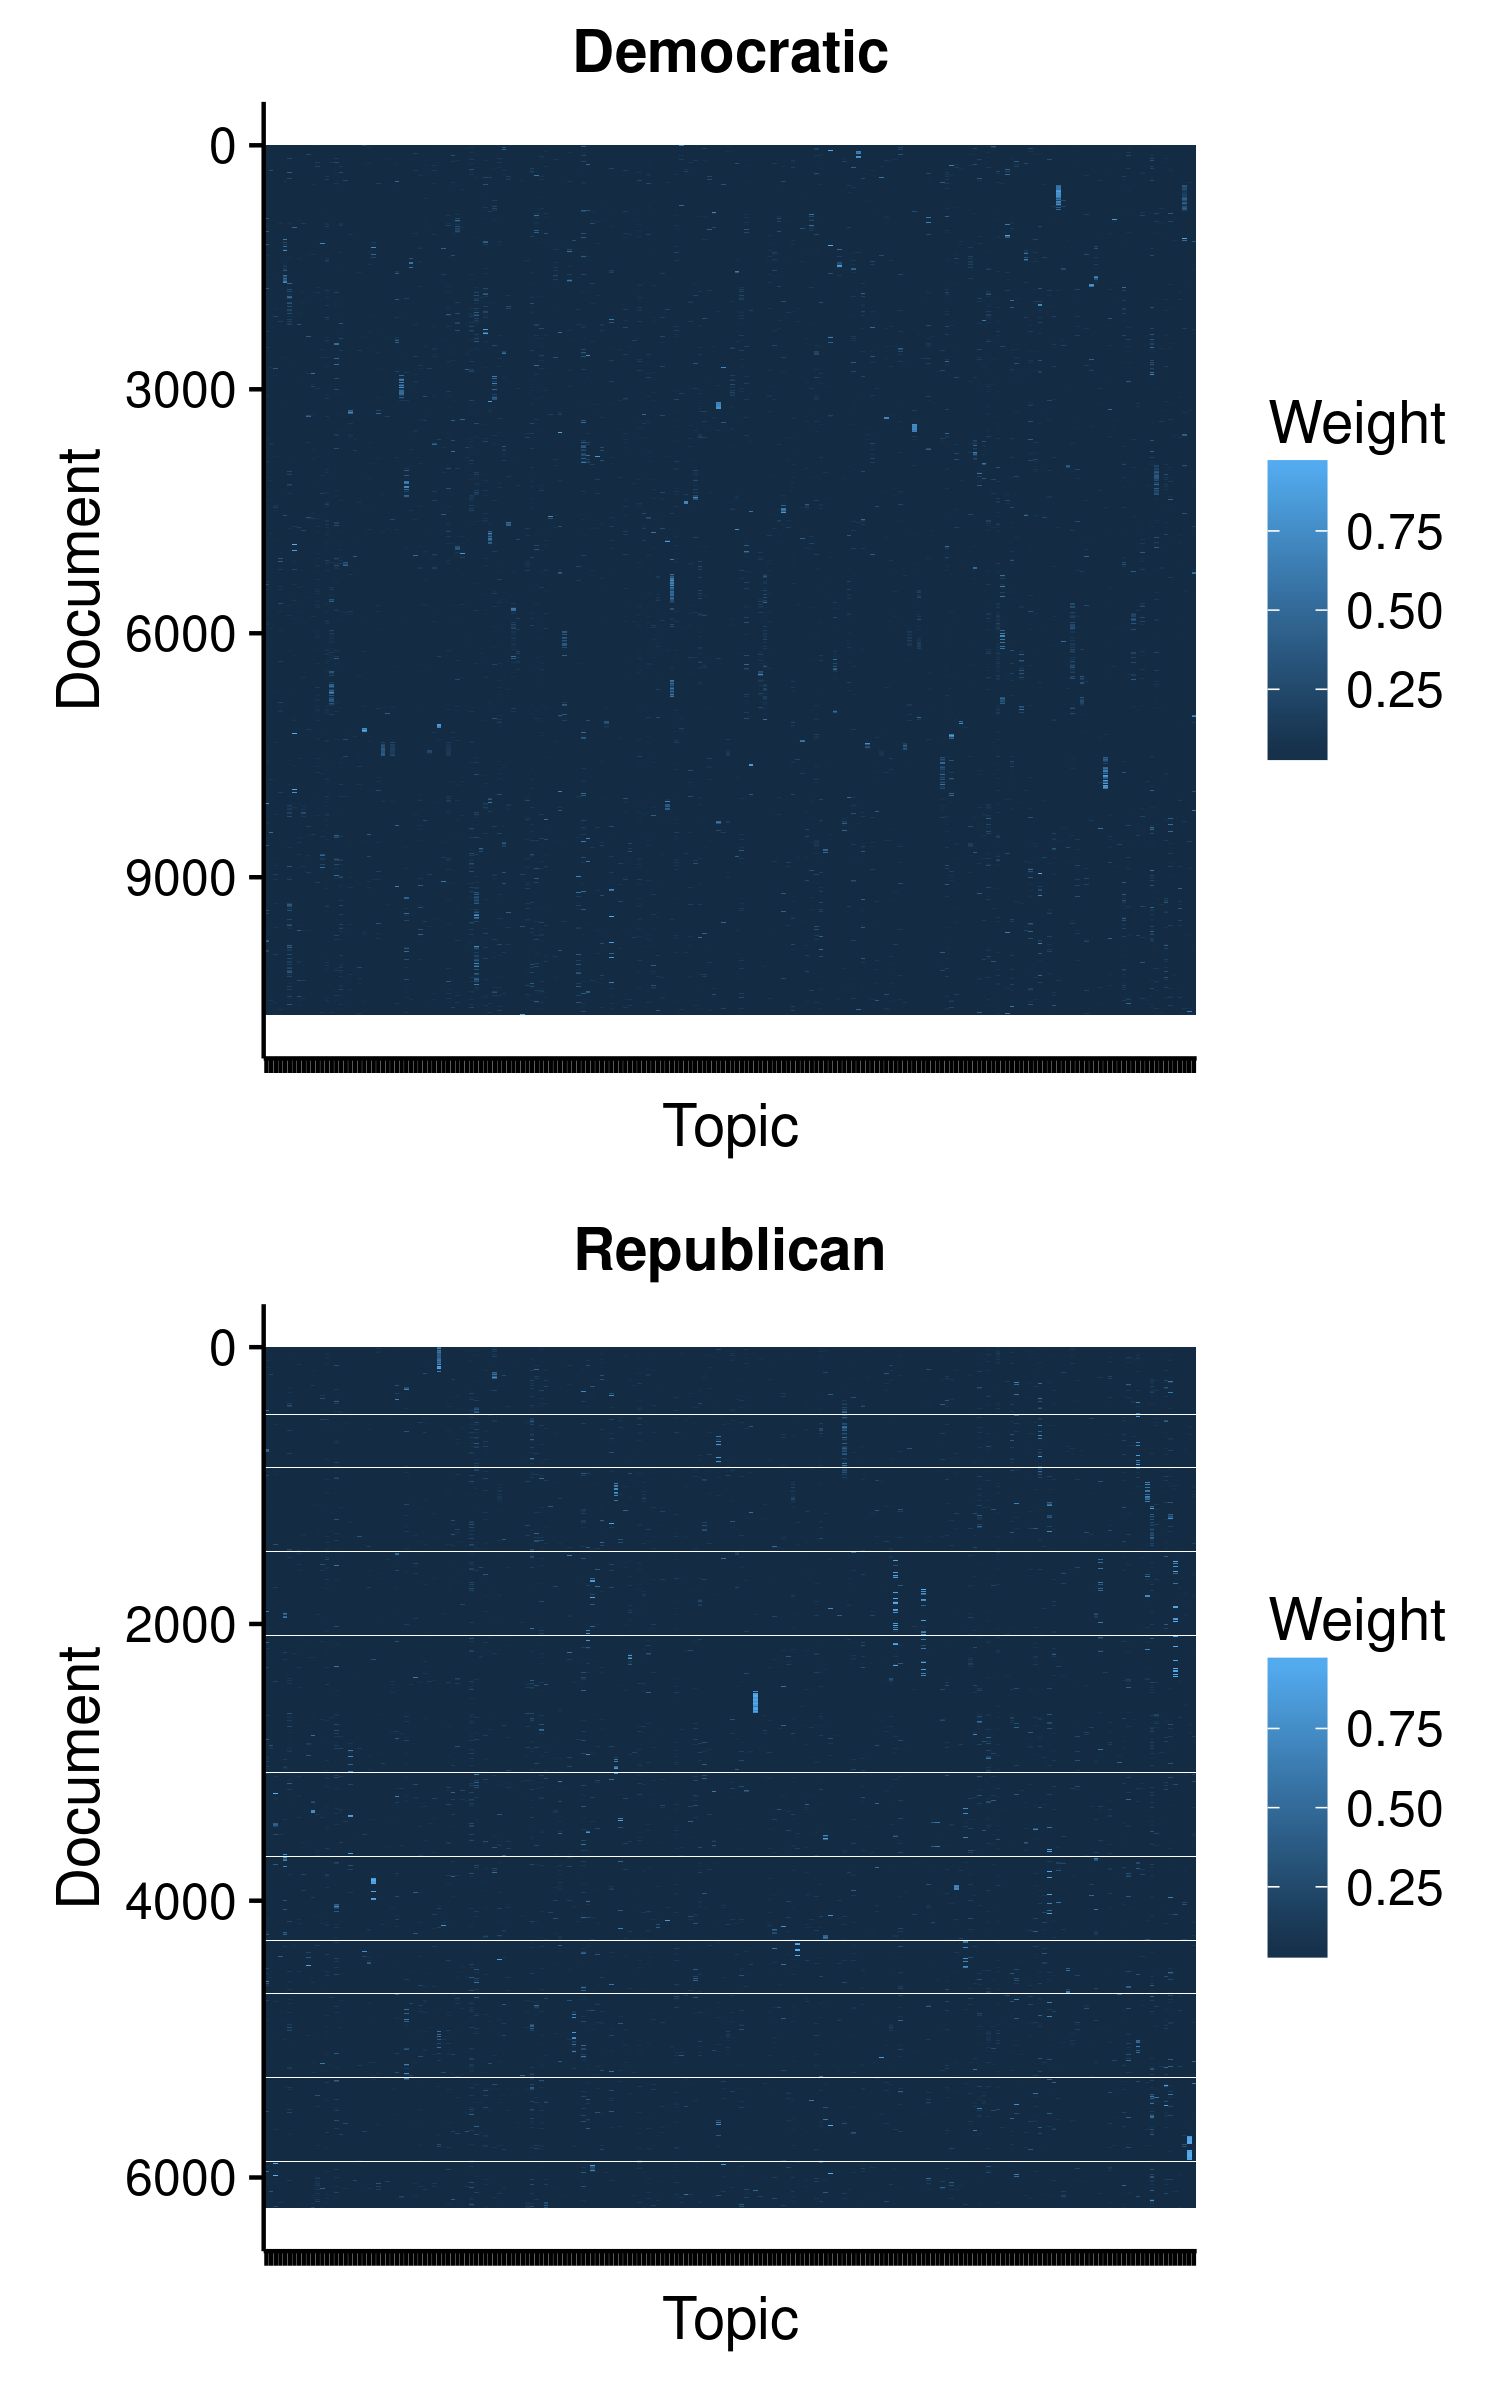
\includegraphics[width=0.8\linewidth]{figures/heatmaps_weights_IN.png}
\end{figure}



%Indiana map
\begin{figure}[htp]
	\centering % Using \begin{figure*} makes the figure take up the entire width of the page
	\caption{Cities in the corpus, by partisanship of mayor.}
	\label{indiana_map}
	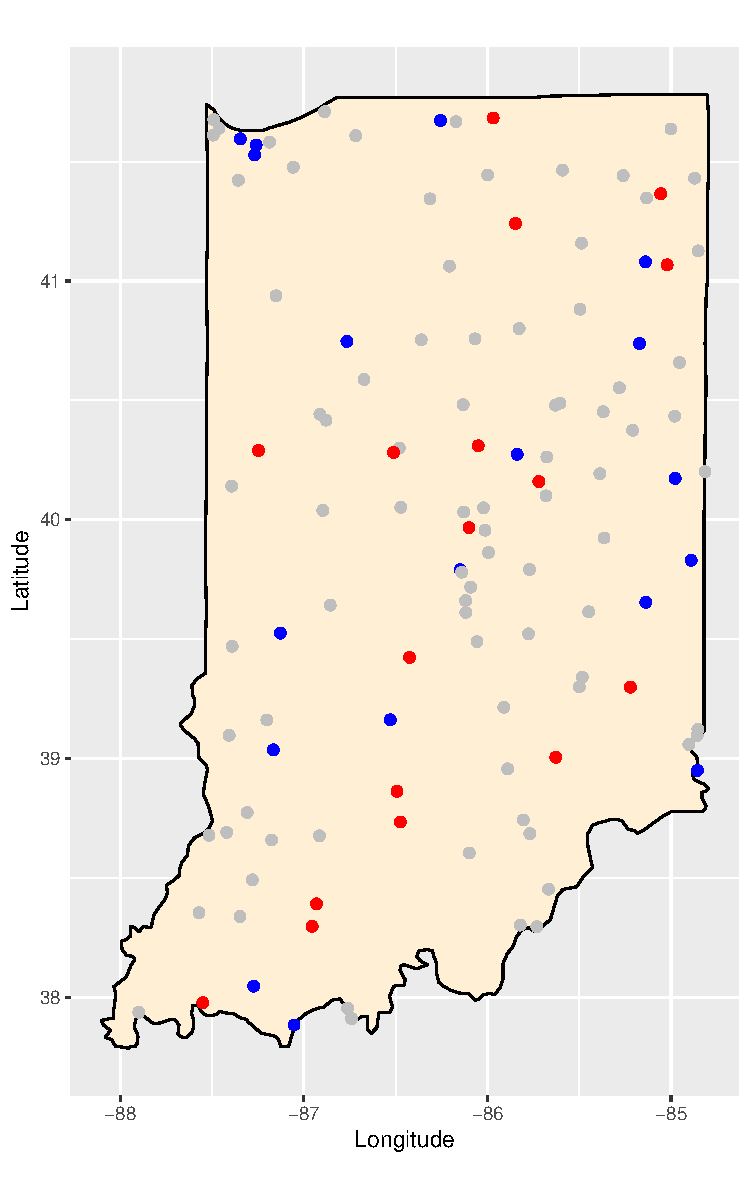
\includegraphics[height=0.75\textheight]{figures/indiana_map.pdf}
\end{figure}

%stm results
\begin{figure}[htp]
	\centering % Using \begin{figure*} makes the figure take up the entire width of the page
	\caption{Results from a structural topic model, displayed as the p-values for each variable for each topic. This would normally be somewhat nonsensical, but here it illustrates why the model does not work.}
	\label{stm_results}
%	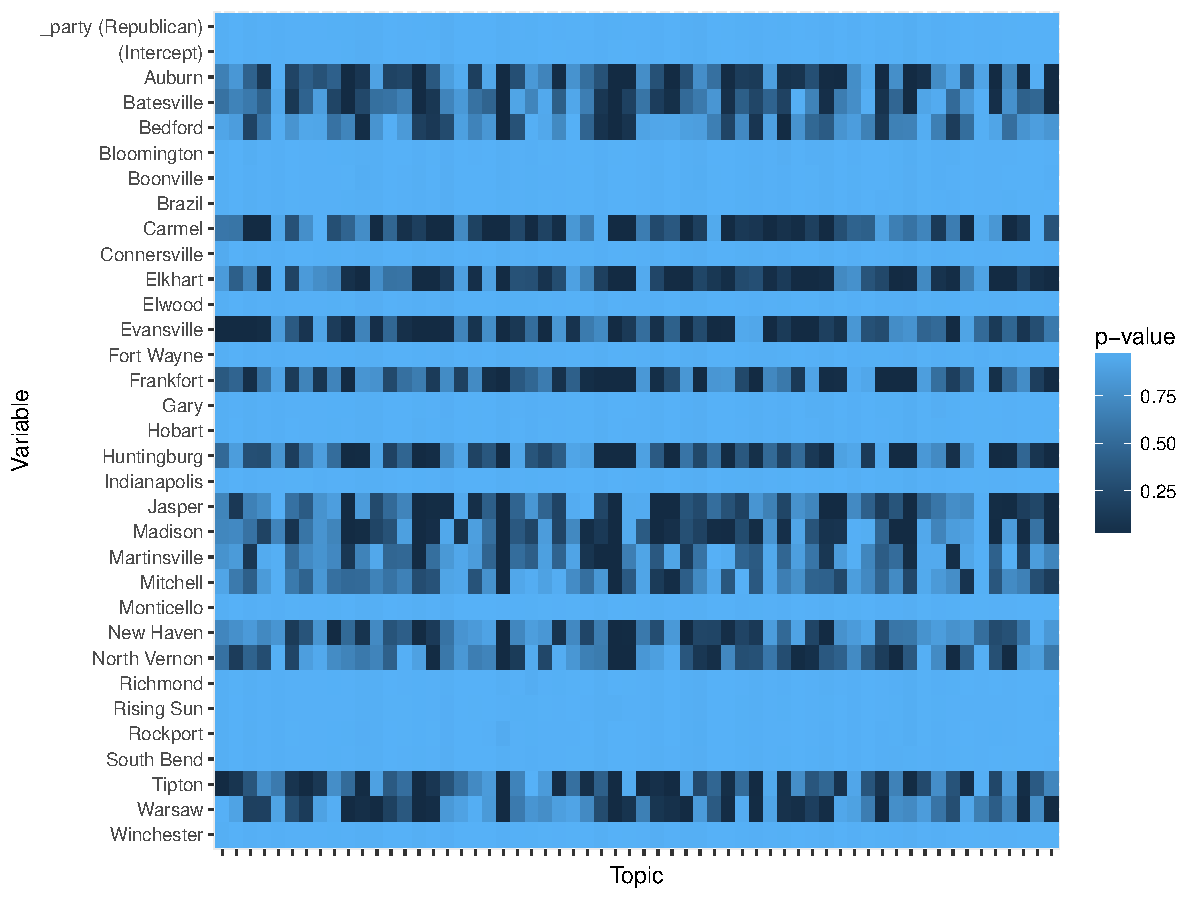
\includegraphics[width=1.1\linewidth]{figures/stm_results.pdf}
\end{figure}



%Partisan top words - topic model Indiana
% latex table generated in R 3.4.1 by xtable 1.8-2 package
% Fri Oct 20 13:14:52 2017
\begin{table}[ht]
\centering
\begingroup\fontsize{9pt}{10pt}\selectfont
\begin{tabular}{lrlr}
  \hline
Word (D) & Instances (D) & Word (R) & Instances (R) \\ 
  \hline
city & 42493 & will & 53761 \\ 
  said & 40480 & city & 36210 \\ 
  county & 39209 & street & 21207 \\ 
  proposal & 29019 & board & 19496 \\ 
  public & 27070 & water & 18637 \\ 
  council & 23492 & plan & 18241 \\ 
  shall & 23162 & public & 14327 \\ 
  department & 22926 & use & 13233 \\ 
  services & 22703 & information & 13062 \\ 
  fund & 21661 & development & 12916 \\ 
  will & 20697 & department & 11554 \\ 
  new & 19000 & area & 11270 \\ 
  stated & 18794 & shall & 11247 \\ 
  project & 18538 & fire & 10861 \\ 
  property & 18378 & can & 10748 \\ 
  budget & 16631 & must & 10633 \\ 
  community & 16236 & park & 10493 \\ 
  asked & 16231 & building & 10356 \\ 
  tax & 14549 & motion & 10168 \\ 
  board & 14363 & ordinance & 9625 \\ 
  state & 13964 & request & 9512 \\ 
  office & 13818 & council & 9098 \\ 
  program & 13536 & community & 9072 \\ 
  year & 13376 & meeting & 8990 \\ 
  service & 13312 & ave & 8555 \\ 
  provide & 13138 & service & 8040 \\ 
  one & 13066 & construction & 7999 \\ 
  section & 12669 & one & 7885 \\ 
  work & 11986 & property & 7741 \\ 
  information & 11886 & also & 7492 \\ 
  development & 11854 & per & 7442 \\ 
  committee & 11802 & required & 7407 \\ 
  district & 11584 & home & 7334 \\ 
  time & 11466 & center & 7316 \\ 
  total & 10965 & made & 7301 \\ 
  general & 10731 & site & 7279 \\ 
  parks & 10704 & business & 7222 \\ 
  system & 10668 & time & 7157 \\ 
  digest & 10481 & services & 7140 \\ 
  police & 10474 & housing & 7111 \\ 
  management & 10433 & new & 7006 \\ 
  park & 10356 & within & 6910 \\ 
  also & 10112 & date & 6818 \\ 
  division & 9964 & year & 6768 \\ 
  street & 9853 & following & 6754 \\ 
  resolution & 9768 & road & 6629 \\ 
  contract & 9763 & member & 6450 \\ 
  ordinance & 9456 & inc & 6367 \\ 
  safety & 9362 & number & 6360 \\ 
  code & 9342 & day & 6254 \\ 
   \hline
\end{tabular}
\endgroup
\caption{Top 50 Democratic and Republican words (Indiana), according to LDA. 
             Topic ownership is determined by the ratio of Democratic to Republican tokens in 
             it (both weighted by the total number of tokens per party). The instances of each 
             token type are then summed across all topics owned by the party.} 
\label{tabLDAIN}
\end{table}

 %\ref{tabFightinIN}

%Partisan top words - topic model Louisiana
% latex table generated in R 3.4.1 by xtable 1.8-2 package
% Fri Oct 20 12:46:14 2017
\begin{table}[ht]
\centering
\begingroup\fontsize{9pt}{10pt}\selectfont
\begin{tabular}{lrlr}
  \hline
Word (D) & Instances (D) & Word (R) & Instances (R) \\ 
  \hline
city & 19306 & city & 9930 \\ 
  stream & 13397 & ordinance & 4413 \\ 
  new & 13001 & information & 3756 \\ 
  obj & 10440 & council & 3422 \\ 
  otherwise & 8271 & said & 3301 \\ 
  street & 7990 & plan & 3194 \\ 
  provide & 7647 & department & 2991 \\ 
  district & 7449 & state & 2598 \\ 
  property & 7031 & public & 2594 \\ 
  public & 6864 & meeting & 2392 \\ 
  shall & 6750 & mayor & 2258 \\ 
  respect & 6698 & one & 2166 \\ 
  water & 6085 & application & 2105 \\ 
  thereto & 5686 & development & 2017 \\ 
  development & 5124 & parish & 1809 \\ 
  use & 5086 & can & 1807 \\ 
  ordinance & 4963 & new & 1807 \\ 
  business & 4763 & water & 1780 \\ 
  department & 4757 & program & 1691 \\ 
  community & 4705 & project & 1674 \\ 
  authorizing & 4440 & time & 1648 \\ 
  located & 4315 & code & 1641 \\ 
  mayor & 4266 & year & 1560 \\ 
  length & 4215 & date & 1556 \\ 
  project & 3918 & number & 1548 \\ 
  section & 3863 & name & 1516 \\ 
  service & 3831 & street & 1504 \\ 
  councilman & 3824 & motion & 1500 \\ 
  services & 3782 & day & 1483 \\ 
  zoning & 3771 & park & 1471 \\ 
  parish & 3731 & home & 1469 \\ 
  providing & 3641 & address & 1415 \\ 
  one & 3636 & office & 1408 \\ 
  system & 3617 & amount & 1392 \\ 
  building & 3607 & ave & 1384 \\ 
  can & 3557 & budget & 1382 \\ 
  code & 3532 & please & 1375 \\ 
  office & 3305 & community & 1334 \\ 
  drive & 3223 & area & 1326 \\ 
  work & 3171 & contact & 1319 \\ 
  permit & 3165 & emergency & 1308 \\ 
  following & 3153 & summary & 1282 \\ 
  within & 3123 & also & 1271 \\ 
  must & 3088 & make & 1265 \\ 
  plan & 3064 & two & 1224 \\ 
  neighborhood & 3048 & work & 1213 \\ 
  construction & 3016 & fire & 1184 \\ 
  chapter & 2973 & bid & 1134 \\ 
  ordinances & 2885 & planning & 1124 \\ 
  fire & 2878 & people & 1108 \\ 
   \hline
\end{tabular}
\endgroup
\caption{Top 50 Democratic and Republican words (Louisiana), according to LDA. 
             Topic ownership is determined by the ratio of Democratic to Republican tokens in 
             it (both weighted by the total number of tokens per party). The instances of each 
             token type are then summed across all topics owned by the party.} 
\label{tabLDALA}
\end{table}

 %tabLDALA

%Partisan top words - stm Indiana
%% latex table generated in R 3.4.2 by xtable 1.8-2 package
% Tue Nov  7 21:46:14 2017
\begin{table}[ht]
\centering
\caption{Top 50 Democratic and Republican words (Indiana), according to STM. 
             The words are the top words for the most Democratic/Republican topic, determined
             by the size (and significance) of the coefficient of the party covariate.} 
\label{tabSTMIN}
\begingroup\footnotesize
\begin{tabular}{ccr|ccr}
  \toprule 
 \multicolumn{3}{c}{\textbf{Democratic}} & \multicolumn{3}{c}{\textbf{Republican}} \\
 \cmidrule(l){1-3} \cmidrule(l){4-6}
  Topic & Coefficient & Word & Topic & Coefficient & Word \\
 \midrule 
   59 & -0.026 & fort &   28 & 0.024 & motion \\ 
    59 & -0.026 & citi &   28 & 0.024 & second \\ 
    59 & -0.026 & ordin &   28 & 0.024 & made \\ 
    59 & -0.026 & approv &   28 & 0.024 & approv \\ 
    59 & -0.026 & purchas &   28 & 0.024 & mayor \\ 
    59 & -0.026 & depart &   28 & 0.024 & present \\ 
    59 & -0.026 & properti &   28 & 0.024 & state \\ 
    59 & -0.026 & will &   28 & 0.024 & will \\ 
    59 & -0.026 & resolut &   28 & 0.024 & citi \\ 
    59 & -0.026 & contract &   28 & 0.024 & council \\ 
   \cmidrule(l){1-3} \cmidrule(l){4-6}
  50 & -0.019 & propos &   11 & 0.019 & plan \\ 
    50 & -0.019 & author &   11 & 0.019 & zone \\ 
    50 & -0.019 & district &   11 & 0.019 & applic \\ 
    50 & -0.019 & street &   11 & 0.019 & properti \\ 
    50 & -0.019 & public &   11 & 0.019 & approv \\ 
    50 & -0.019 & control &   11 & 0.019 & sign \\ 
    50 & -0.019 & amend &   11 & 0.019 & site \\ 
    50 & -0.019 & intersect &   11 & 0.019 & locat \\ 
    50 & -0.019 & counti &   11 & 0.019 & commiss \\ 
    50 & -0.019 & committe &   11 & 0.019 & file \\ 
   \cmidrule(l){1-3} \cmidrule(l){4-6}
  42 & -0.018 & said &    2 & 0.019 & inc \\ 
    42 & -0.018 & ask &    2 & 0.019 & electr \\ 
    42 & -0.018 & state &    2 & 0.019 & build \\ 
    42 & -0.018 & will &    2 & 0.019 & construct \\ 
    42 & -0.018 & chair &    2 & 0.019 & home \\ 
    42 & -0.018 & propos &    2 & 0.019 & street \\ 
    42 & -0.018 & year &    2 & 0.019 & meridian \\ 
    42 & -0.018 & move &    2 & 0.019 & servic \\ 
    42 & -0.018 & need &    2 & 0.019 & west \\ 
    42 & -0.018 & council &    2 & 0.019 & main \\ 
   \cmidrule(l){1-3} \cmidrule(l){4-6}
  16 & -0.018 & prosecutor &   27 & 0.016 & request \\ 
    16 & -0.018 & charg &   27 & 0.016 & board \\ 
    16 & -0.018 & feloni &   27 & 0.016 & member \\ 
    16 & -0.018 & counti &   27 & 0.016 & servic \\ 
    16 & -0.018 & case &   27 & 0.016 & street \\ 
    16 & -0.018 & crime &   27 & 0.016 & approv \\ 
    16 & -0.018 & crimin &   27 & 0.016 & purchas \\ 
    16 & -0.018 & offic &   27 & 0.016 & citi \\ 
    16 & -0.018 & victim &   27 & 0.016 & move \\ 
    16 & -0.018 & sentenc &   27 & 0.016 & good \\ 
   \cmidrule(l){1-3} \cmidrule(l){4-6}
  13 & -0.018 & digest &   35 & 0.016 & council \\ 
    13 & -0.018 & introduc &   35 & 0.016 & citi \\ 
    13 & -0.018 & author &   35 & 0.016 & ordin \\ 
    13 & -0.018 & counti &   35 & 0.016 & common \\ 
    13 & -0.018 & appoint &   35 & 0.016 & councilor \\ 
    13 & -0.018 & board &   35 & 0.016 & amend \\ 
    13 & -0.018 & approv &   35 & 0.016 & resolut \\ 
    13 & -0.018 & district &   35 & 0.016 & adopt \\ 
    13 & -0.018 & fund &   35 & 0.016 & wherea \\ 
    13 & -0.018 & street &   35 & 0.016 & approv \\ 
   \bottomrule 
\end{tabular}
\endgroup
\end{table}

 %\ref{tabSTMLA}

%Partisan top words - stm Louisiana
%% latex table generated in R 3.4.2 by xtable 1.8-2 package
% Sun Oct 29 16:12:17 2017
\begin{table}[ht]
\centering
\begingroup\fontsize{9pt}{10pt}\selectfont
\begin{tabular}{rrlrrl}
  \hline
demTopic & demTopicCoeff & Democratic & repTopic & repTopicCoeff & Republican \\ 
  \hline
   1 & -0.171 & stream &   49 & 0.095 & event \\ 
     1 & -0.171 & obj &   49 & 0.095 & music \\ 
     1 & -0.171 & interpol &   49 & 0.095 & church \\ 
     1 & -0.171 & baa &   49 & 0.095 & inform \\ 
     1 & -0.171 & matrix &   49 & 0.095 & show \\ 
     1 & -0.171 & metadata &   49 & 0.095 & park \\ 
     1 & -0.171 & hum &   49 & 0.095 & market \\ 
     1 & -0.171 & gym &   49 & 0.095 & visit \\ 
     1 & -0.171 & rid &   49 & 0.095 & year \\ 
     1 & -0.171 & yep &   49 & 0.095 & featur \\ 
    15 & -0.045 & length &   13 & 0.093 & said \\ 
    15 & -0.045 & root &   13 & 0.093 & work \\ 
    15 & -0.045 & predictor &   13 & 0.093 & citi \\ 
    15 & -0.045 & eye &   13 & 0.093 & depart \\ 
    15 & -0.045 & word &   13 & 0.093 & airport \\ 
    15 & -0.045 & acrobat &   13 & 0.093 & code \\ 
    15 & -0.045 & adob &   13 & 0.093 & offici \\ 
    15 & -0.045 & ash &   13 & 0.093 & resid \\ 
    15 & -0.045 & rang &   13 & 0.093 & mayor \\ 
    15 & -0.045 & vet &   13 & 0.093 & continu \\ 
    57 & -0.044 & otherwis &   56 & 0.064 & ordin \\ 
    57 & -0.044 & provid &   56 & 0.064 & summari \\ 
    57 & -0.044 & respect &   56 & 0.064 & amount \\ 
    57 & -0.044 & thereto &   56 & 0.064 & citi \\ 
    57 & -0.044 & citi &   56 & 0.064 & bid \\ 
    57 & -0.044 & author &   56 & 0.064 & depart \\ 
    57 & -0.044 & ordin &   56 & 0.064 & motion \\ 
    57 & -0.044 & amend &   56 & 0.064 & approv \\ 
    57 & -0.044 & district &   56 & 0.064 & public \\ 
    57 & -0.044 & locat &   56 & 0.064 & contract \\ 
    41 & -0.017 & pdf &   12 & 0.049 & flood \\ 
    41 & -0.017 & content &   12 & 0.049 & emerg \\ 
    41 & -0.017 & type &   12 & 0.049 & storm \\ 
    41 & -0.017 & width &   12 & 0.049 & disast \\ 
    41 & -0.017 & text &   12 & 0.049 & weather \\ 
    41 & -0.017 & resourc &   12 & 0.049 & hurrican \\ 
    41 & -0.017 & parent &   12 & 0.049 & can \\ 
    41 & -0.017 & filter &   12 & 0.049 & area \\ 
    41 & -0.017 & font &   12 & 0.049 & busi \\ 
    41 & -0.017 & page &   12 & 0.049 & inform \\ 
     5 & -0.017 & polic &    3 & 0.022 & councilman \\ 
     5 & -0.017 & crime &    3 & 0.022 & want \\ 
     5 & -0.017 & offic &    3 & 0.022 & said \\ 
     5 & -0.017 & investig &    3 & 0.022 & just \\ 
     5 & -0.017 & arrest &    3 & 0.022 & know \\ 
     5 & -0.017 & suspect &    3 & 0.022 & get \\ 
     5 & -0.017 & victim &    3 & 0.022 & like \\ 
     5 & -0.017 & report &    3 & 0.022 & citi \\ 
     5 & -0.017 & block &    3 & 0.022 & can \\ 
     5 & -0.017 & vehicl &    3 & 0.022 & come \\ 
   \hline
\end{tabular}
\endgroup
\caption{Top 50 Democratic and Republican words (Louisiana), according to STM. 
             The words are the top words for the most Democratic/Republican topic, determined
             by the size (and significance) of the coefficient of the party covariate.} 
\label{tabSTMLA}
\end{table}

 %\ref{tabSTMLA}


%Some basic descriptive statistics of documents by party
% latex table generated in R 3.4.1 by xtable 1.8-2 package
% Fri Oct 20 13:41:38 2017
\begin{table}[ht]
\centering
\begin{tabular}{rrr}
  \hline
 & Democratic & Republican \\ 
  \hline
Cities & 15 & 17 \\ 
  Documents & 10257 & 5859 \\ 
  Tokens & 6101752 & 2310072 \\ 
  Token assignments & 6006202 & 2259362 \\ 
  Topics & 103 & 97 \\ 
   \hline
\end{tabular}
\caption{Descriptive statistics for Indiana. ``Tokens'' describes the number
             of words in each party's documents, ``token assignments'' the tokens assigned
             to each party in the topic model depending on the ratio of Democratic to Republican 
             tokens in it (both weighted by the total number of tokens per party).} 
\label{tabDescriptiveIN}
\end{table}



%Some basic descriptive statistics of documents by party
% latex table generated in R 3.4.1 by xtable 1.8-2 package
% Fri Oct 20 13:53:50 2017
\begin{table}[ht]
\centering
\begin{tabular}{rrr}
  \hline
 & Democratic & Republican \\ 
  \hline
Cities & 11 & 7 \\ 
  Documents & 6287 & 1327 \\ 
  Tokens & 1955198 & 322915 \\ 
  Token assignments & 1789373 & 314628 \\ 
  Topics & 143 & 57 \\ 
   \hline
\end{tabular}
\caption{Descriptive statistics for Louisiana. ``Tokens'' describes the number
             of words in each party's documents, ``token assignments'' the tokens assigned
             to each party in the topic model depending on the ratio of Democratic to Republican 
             tokens in it (both weighted by the total number of tokens per party).} 
\label{tabDescriptiveLA}
\end{table}



%fightin words results
\begin{figure}[htp]
	\centering % Using \begin{figure*} makes the figure take up the entire width of the page
	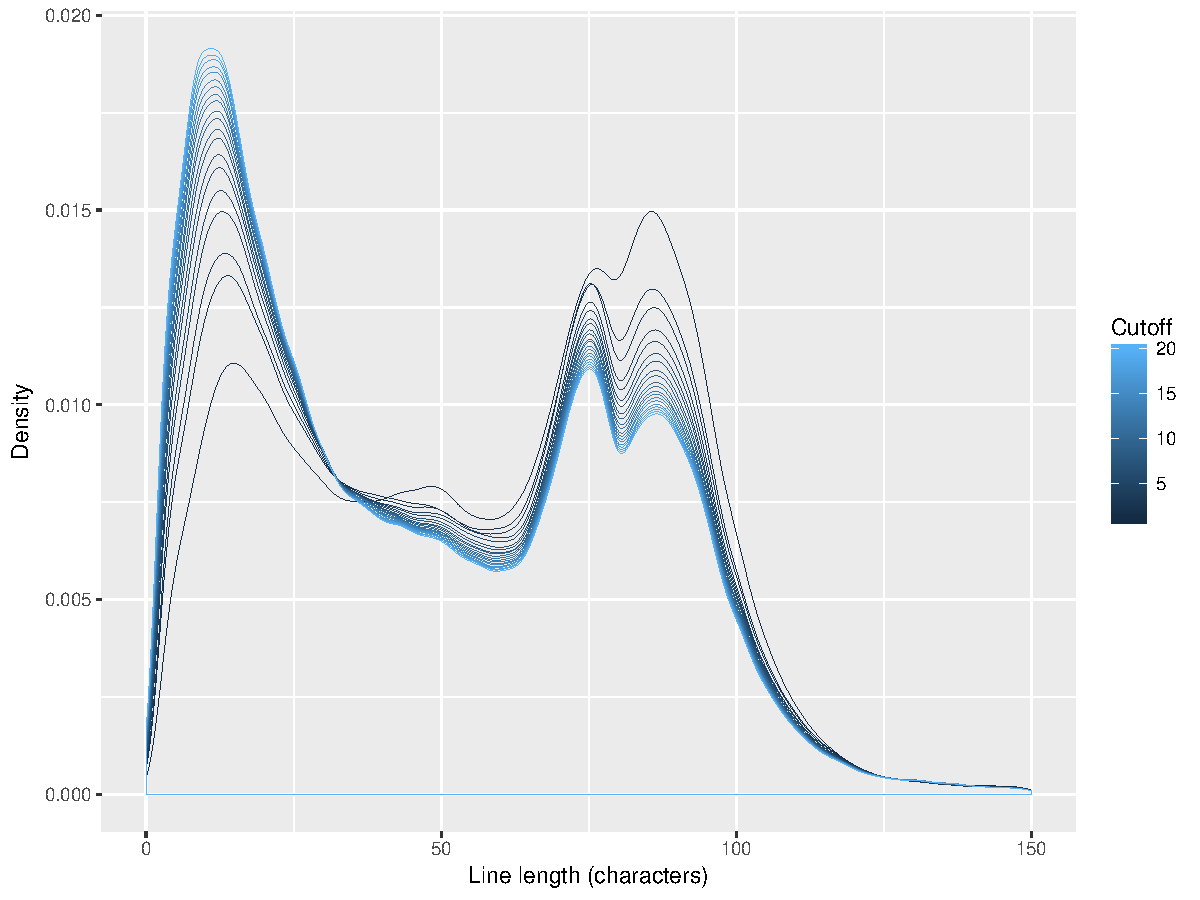
\includegraphics[width=\linewidth]{figures/linesCutoffIN.pdf}
		\caption{Total number of lines retained at a given threshold for removing duplicated lines. For example, at x = 10, all lines occurring more than 10 times within a city's documents are removed.}
	\label{linesCutoff}
\end{figure}


\section{Ground truth test}
In the realm of public administration, the notion that the partisan leaning of mayors might have an effect on how they run their cities is still frowned upon to some extent. Perceived more as managers than politicians, they have been portrayed as the last bastion of non-partisanship in America, and in many cases, also style themselves that way \citep{Dovere2018}. However, the aspirations some mayors have shown towards higher offices - in some cases even the presidency - reveal that they are not quite as above the fray as some may believe them to be. One of the most vicious and blatantly partisan cleavages in current U.S. politics - the debate surrounding sanctuary cities - has seen mayors in a central role. Research into local politics has shown that partisan elections consistently have greater turnout \citep{Schaffner2001}. When voters are denied this cue, they make use of other, and considerably more irrational heuristics, such as name, gender, or occupation of the contenders. Consequently it only makes sense for any office-seeking politician to emphasize their partisanship. Finally, decades of research in political psychology have consistently shown that no matter how hard we try, humans are simply incapable of escaping our partisan biases, a finding that is especially pronounced among elites \citep{Hatemi2011}.

In an effort to underline this fact and remove any doubt about the fact that the partisanship of mayors colors their decision-making, we conduct a ground truth test between our main corpus - the websites of cities - and a second, decidedly more partisan set of texts: the campaign websites of these mayors. As noted above, partisanship has been shown to be a powerful driving force even in local politics, and mayors are incentivized to exploit it. Consequently they are very likely to emphasize conservative/liberal values on this platform. If there is a greater correlation in word use between the cities managed by a party and the campaign websites of its mayors than with those of the other party, evidence for the partisanship of city websites can be established.

Using the same methods as described for our main corpus, we have gathered these sites and then concatenated all of the documents belonging to mayors of the two parties into one ground truth document each. We do the same for the city documents, and the compare the four document collections using cosine similarity. This measure is the cosine between the angle of two vectors, in this case the frequencies of all words in the two vocabularies. Compared to a simple euclidean distance, this has the advantage of accounting for the fact that the two corpora being compared are not necessarily of the same length. The cosine measure between two documents ranges between 0 and 1, 0 signifying absolutely no correlation, and 1 perfect overlap. Figure \ref{groundtruth} shows the result of this test. The expectation is for a greater similarity between Republican cities and the Republican ground truth, than Republican cities and Democratic ground truth - and vice versa. At present however, this does not appear to be the case, presumably because the Republican ground truth consists of 8 documents, and the Democratic one of 290.

%ground truth test
\begin{figure}[htp]
	\centering % Using \begin{figure*} makes the figure take up the entire width of the page
	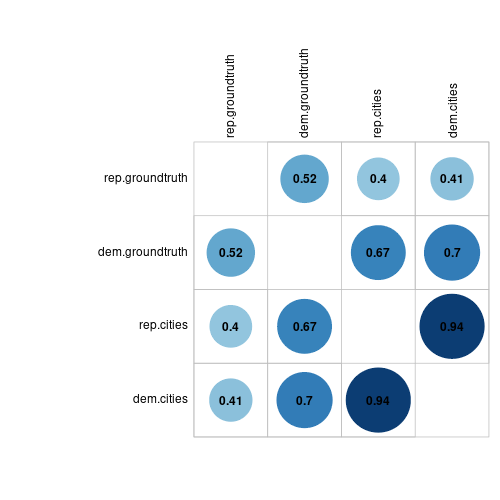
\includegraphics[width=\linewidth]{figures/groundtruth_corrplot.png}
	\caption{Ground truth test. The values are cosine similarities between a pair of document collections.}
	\label{groundtruth}
\end{figure}

%ground truth test
\begin{figure}[htp]
	\centering % Using \begin{figure*} makes the figure take up the entire width of the page
	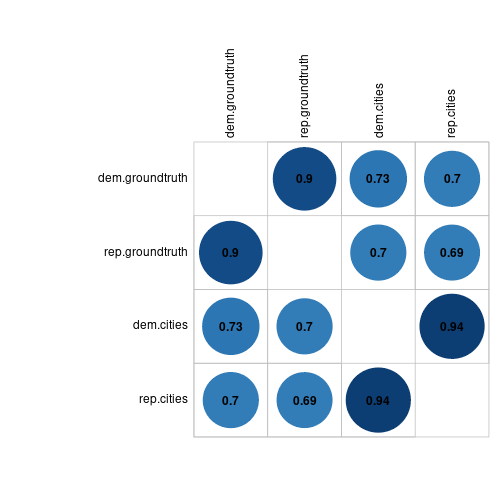
\includegraphics[width=\linewidth]{figures/groundtruth_bs_bigcities_corrplot.png}
	\caption{Ground truth test. The values are cosine similarities between a pair of document collections (top 100 mayors vs. IN and LA).}
	\label{groundtruth}
\end{figure}

%Ground truth test between top100 mayors and IN + LA; with bootstrapped confidence bounds
% label: groundtruth_bootstrapped
% latex table generated in R 3.4.3 by xtable 1.8-2 package
% Tue Feb 13 10:36:40 2018
\begin{table}[ht]
\centering
\begin{tabular}{rllll}
  \hline
 & dem.groundtruth & rep.groundtruth & dem.cities & rep.cities \\ 
  \hline
dem.groundtruth & 1, 1 & 0.807, 0.896 & 0.714, 0.729 & 0.68, 0.698 \\ 
  rep.groundtruth & 0.807, 0.896 & 1, 1 & 0.647, 0.697 & 0.641, 0.693 \\ 
  dem.cities & 0.714, 0.729 & 0.647, 0.697 & 1, 1 & 0.937, 0.944 \\ 
  rep.cities & 0.68, 0.698 & 0.641, 0.693 & 0.937, 0.944 & 1, 1 \\ 
   \hline
\end{tabular}
\caption{Ground truth test, comparing campaign websites of mayors of the 100 largest cities in the US and cities in Indiana and Louisiana. The values are bootstrapped confidence bounds for cosine similarities between concatenated document collections.} 
\label{groundtruth_bootstrapped}
\end{table}




% latex table generated in R 3.4.4 by xtable 1.8-2 package
% Mon Apr 23 14:12:56 2018
\begin{table}[ht]
\centering
\begingroup\scriptsize
\begin{tabular}{lllllll}
  \hline
1 & 2 & 3 & 4 & 5 & 6 & 7 \\ 
  \hline
\cellcolor{red!10}yon & \cellcolor{red!10}borough & \cellcolor{red!10}port & \cellcolor{red!10}waterfront & \cellcolor{red!10}queens & \cellcolor{red!10}boroughs & \cellcolor{red!10}island \\ 
  \cellcolor{blue!10}noise & \cellcolor{blue!10}impacts & \cellcolor{blue!10}mitigation & \cellcolor{blue!10}vibration & \cellcolor{blue!10}ambient & \cellcolor{blue!10}adverse & \cellcolor{blue!10}thresholds \\ 
  \cellcolor{red!10}tax & \cellcolor{red!10}exemption & \cellcolor{red!10}taxes & \cellcolor{red!10}estate & \cellcolor{red!10}assessed & \cellcolor{red!10}real & \cellcolor{red!10}taxpayer \\ 
  \cellcolor{red!10}para & \cellcolor{red!10}personas & \cellcolor{red!10}antes & \cellcolor{red!10}persona & \cellcolor{red!10}horas & \cellcolor{red!10}junta & \cellcolor{red!10}con \\ 
  \cellcolor{blue!10}election & \cellcolor{blue!10}ethics & \cellcolor{blue!10}appointed & \cellcolor{blue!10}elections & \cellcolor{blue!10}ballot & \cellcolor{blue!10}charter & \cellcolor{blue!10}elected \\ 
  \cellcolor{red!10}wetland & \cellcolor{red!10}habitats & \cellcolor{red!10}riparian & \cellcolor{red!10}habitat & \cellcolor{red!10}wetlands & \cellcolor{red!10}tidal & \cellcolor{red!10}freshwater \\ 
  \cellcolor{blue!10}parking & \cellcolor{blue!10}bus & \cellcolor{blue!10}transit & \cellcolor{blue!10}mall & \cellcolor{blue!10}buses & \cellcolor{blue!10}campus & \cellcolor{blue!10}arena \\ 
  \cellcolor{red!30}click & \cellcolor{red!30}download & \cellcolor{red!30}online & \cellcolor{red!30}please & \cellcolor{red!30}email & \cellcolor{red!30}website & \cellcolor{red!30}visit \\ 
  \cellcolor{blue!10}draft & \cellcolor{blue!10}comments & \cellcolor{blue!10}comment & \cellcolor{blue!10}meetings & \cellcolor{blue!10}update & \cellcolor{blue!10}presentation & \cellcolor{blue!10}briefing \\ 
  \cellcolor{blue!10}ave & \cellcolor{blue!10}blvd & \cellcolor{blue!10}glen & \cellcolor{blue!10}pkwy & \cellcolor{blue!10}hwy & \cellcolor{blue!10}cove & \cellcolor{blue!10}fwy \\ 
  \cellcolor{blue!20}neighborhoods & \cellcolor{blue!20}strategy & \cellcolor{blue!20}vision & \cellcolor{blue!20}strategies & \cellcolor{blue!20}businesses & \cellcolor{blue!20}opportunities & \cellcolor{blue!20}vibrant \\ 
  \cellcolor{white}bid & \cellcolor{white}contract & \cellcolor{white}invoices & \cellcolor{white}procurement & \cellcolor{white}purchasing & \cellcolor{white}bids & \cellcolor{white}vendor \\ 
  \cellcolor{white}marijuana & \cellcolor{white}cannabis & \cellcolor{white}licensee & \cellcolor{white}taxicab & \cellcolor{white}license & \cellcolor{white}mischief & \cellcolor{white}citation \\ 
  \cellcolor{blue!10}complaint & \cellcolor{blue!10}discrimination & \cellcolor{blue!10}defendants & \cellcolor{blue!10}bankruptcy & \cellcolor{blue!10}trial & \cellcolor{blue!10}harassment & \cellcolor{blue!10}defendant \\ 
  \cellcolor{red!10}rouge & \cellcolor{red!10}baton & \cellcolor{red!10}foods & \cellcolor{red!10}parish & \cellcolor{red!10}vegetables & \cellcolor{red!10}vending & \cellcolor{red!10}cooked \\ 
  \cellcolor{red!10}child & \cellcolor{red!10}violence & \cellcolor{red!10}abuse & \cellcolor{red!10}mental & \cellcolor{red!10}clients & \cellcolor{red!10}inmates & \cellcolor{red!10}homelessness \\ 
  \cellcolor{red!10}applicants & \cellcolor{red!10}landlord & \cellcolor{red!10}tenant & \cellcolor{red!10}rent & \cellcolor{red!10}exam & \cellcolor{red!10}tenants & \cellcolor{red!10}applications \\ 
  \cellcolor{red!10}think & \cellcolor{red!10}say & \cellcolor{red!10}really & \cellcolor{red!10}thing & \cellcolor{red!10}okay & \cellcolor{red!10}got & \cellcolor{red!10}maybe \\ 
  \cellcolor{blue!20}setback & \cellcolor{blue!20}fence & \cellcolor{blue!20}yard & \cellcolor{blue!20}zoned & \cellcolor{blue!20}front & \cellcolor{blue!20}height & \cellcolor{blue!20}accessory \\ 
  \cellcolor{red!10}shall & \cellcolor{red!10}subsection & \cellcolor{red!10}article & \cellcolor{red!10}provisions & \cellcolor{red!10}pursuant & \cellcolor{red!10}thereof & \cellcolor{red!10}forth \\ 
  \cellcolor{red!20}explained & \cellcolor{red!20}asked & \cellcolor{red!20}said & \cellcolor{red!20}legislator & \cellcolor{red!20}commented & \cellcolor{red!20}advised & \cellcolor{red!20}leg \\ 
  \cellcolor{blue!10}respondents & \cellcolor{blue!10}census & \cellcolor{blue!10}population & \cellcolor{blue!10}compared & \cellcolor{blue!10}average & \cellcolor{blue!10}trends & \cellcolor{blue!10}comparison \\ 
  \cellcolor{red!20}infection & \cellcolor{red!20}symptoms & \cellcolor{red!20}breastfeeding & \cellcolor{red!20}syphilis & \cellcolor{red!20}doses & \cellcolor{red!20}asthma & \cellcolor{red!20}tuberculosis \\ 
  \cellcolor{red!20}yes & \cellcolor{red!20}name & \cellcolor{red!20}signature & \cellcolor{red!20}mailing & \cellcolor{red!20}zip & \cellcolor{red!20}attach & \cellcolor{red!20}form \\ 
  \cellcolor{red!30}games & \cellcolor{red!30}tournament & \cellcolor{red!30}swim & \cellcolor{red!30}players & \cellcolor{red!30}player & \cellcolor{red!30}camp & \cellcolor{red!30}game \\ 
  \cellcolor{blue!10}goals & \cellcolor{blue!10}implementation & \cellcolor{blue!10}policies & \cellcolor{blue!10}policy & \cellcolor{blue!10}specific & \cellcolor{blue!10}implement & \cellcolor{blue!10}comprehensive \\ 
  \cellcolor{red!20}ems & \cellcolor{red!20}fires & \cellcolor{red!20}preparedness & \cellcolor{red!20}disaster & \cellcolor{red!20}evacuation & \cellcolor{red!20}fire & \cellcolor{red!20}firefighters \\ 
  \cellcolor{red!10}subcontractor & \cellcolor{red!10}subcontractors & \cellcolor{red!10}agrees & \cellcolor{red!10}proposer & \cellcolor{red!10}contractor & \cellcolor{red!10}grantee & \cellcolor{red!10}breach \\ 
  \cellcolor{blue!10}realm & \cellcolor{blue!10}massing & \cellcolor{blue!10}facades & \cellcolor{blue!10}entrances & \cellcolor{blue!10}plazas & \cellcolor{blue!10}elements & \cellcolor{blue!10}proponents \\ 
  \cellcolor{blue!10}employee & \cellcolor{blue!10}allegation & \cellcolor{blue!10}overtime & \cellcolor{blue!10}named & \cellcolor{blue!10}leave & \cellcolor{blue!10}grievance & \cellcolor{blue!10}wage \\ 
  \cellcolor{blue!10}parks & \cellcolor{blue!10}playground & \cellcolor{blue!10}beach & \cellcolor{blue!10}park & \cellcolor{blue!10}picnic & \cellcolor{blue!10}marina & \cellcolor{blue!10}trails \\ 
  \cellcolor{blue!10}lanes & \cellcolor{blue!10}bicycle & \cellcolor{blue!10}bike & \cellcolor{blue!10}intersections & \cellcolor{blue!10}bicyclists & \cellcolor{blue!10}roadway & \cellcolor{blue!10}pedestrians \\ 
  \cellcolor{blue!20}absent & \cellcolor{blue!20}aye & \cellcolor{blue!20}khan & \cellcolor{blue!20}voting & \cellcolor{blue!20}berry & \cellcolor{blue!20}nays & \cellcolor{blue!20}tagged \\ 
  \cellcolor{blue!20}budget & \cellcolor{blue!20}revenue & \cellcolor{blue!20}million & \cellcolor{blue!20}revenues & \cellcolor{blue!20}budgeted & \cellcolor{blue!20}fund & \cellcolor{blue!20}expenditures \\ 
  \cellcolor{blue!10}whereas & \cellcolor{blue!10}resolution & \cellcolor{blue!10}amending & \cellcolor{blue!10}resolved & \cellcolor{blue!10}hereby & \cellcolor{blue!10}authorizes & \cellcolor{blue!10}digest \\ 
  \cellcolor{blue!10}assets & \cellcolor{blue!10}statements & \cellcolor{blue!10}governmental & \cellcolor{blue!10}accounting & \cellcolor{blue!10}liabilities & \cellcolor{blue!10}net & \cellcolor{blue!10}financial \\ 
  \cellcolor{red!30}honored & \cellcolor{red!30}joined & \cellcolor{red!30}proud & \cellcolor{red!30}fort & \cellcolor{red!30}announces & \cellcolor{red!30}won & \cellcolor{red!30}worth \\ 
  \cellcolor{white}analyst & \cellcolor{white}technician & \cellcolor{white}specialist & \cellcolor{white}performs & \cellcolor{white}prepares & \cellcolor{white}coordinates & \cellcolor{white}assists \\ 
  \cellcolor{white}server & \cellcolor{white}wireless & \cellcolor{white}software & \cellcolor{white}aircraft & \cellcolor{white}servers & \cellcolor{white}airport & \cellcolor{white}technology \\ 
  \cellcolor{blue!10}improvements & \cellcolor{blue!10}project & \cellcolor{blue!10}projects & \cellcolor{blue!10}phase & \cellcolor{blue!10}replacement & \cellcolor{blue!10}reconstruction & \cellcolor{blue!10}upgrades \\ 
  \cellcolor{red!10}recycling & \cellcolor{red!10}recycle & \cellcolor{red!10}garbage & \cellcolor{red!10}bags & \cellcolor{red!10}waste & \cellcolor{red!10}recyclable & \cellcolor{red!10}recyclables \\ 
  \cellcolor{blue!10}housing & \cellcolor{blue!10}affordable & \cellcolor{blue!10}households & \cellcolor{blue!10}affordability & \cellcolor{blue!10}income & \cellcolor{blue!10}moderate & \cellcolor{blue!10}homeless \\ 
  \cellcolor{red!20}effluent & \cellcolor{red!20}wastewater & \cellcolor{red!20}discharges & \cellcolor{red!20}contaminants & \cellcolor{red!20}sludge & \cellcolor{red!20}infiltration & \cellcolor{red!20}solids \\ 
  \cellcolor{red!10}fee & \cellcolor{red!10}permit & \cellcolor{red!10}inspection & \cellcolor{red!10}permits & \cellcolor{red!10}inspections & \cellcolor{red!10}fees & \cellcolor{red!10}occupancy \\ 
  \cellcolor{blue!10}uses & \cellcolor{blue!10}mixed & \cellcolor{blue!10}density & \cellcolor{blue!10}land & \cellcolor{blue!10}industrial & \cellcolor{blue!10}residential & \cellcolor{blue!10}commercial \\ 
  \cellcolor{red!10}energy & \cellcolor{red!10}renewable & \cellcolor{red!10}coal & \cellcolor{red!10}electricity & \cellcolor{red!10}climate & \cellcolor{red!10}solar & \cellcolor{red!10}greenhouse \\ 
  \cellcolor{blue!10}bonds & \cellcolor{blue!10}refunding & \cellcolor{blue!10}securities & \cellcolor{blue!10}bond & \cellcolor{blue!10}debt & \cellcolor{blue!10}issuer & \cellcolor{blue!10}maturity \\ 
  \cellcolor{red!20}artists & \cellcolor{red!20}artist & \cellcolor{red!20}performances & \cellcolor{red!20}music & \cellcolor{red!20}orchestra & \cellcolor{red!20}symphony & \cellcolor{red!20}arts \\ 
  \cellcolor{blue!80}arrested & \cellcolor{blue!80}suspect & \cellcolor{blue!80}homicide & \cellcolor{blue!80}suspects & \cellcolor{blue!80}shooting & \cellcolor{blue!80}sergeant & \cellcolor{blue!80}arrests \\ 
  \cellcolor{white}retiree & \cellcolor{white}actuarial & \cellcolor{white}retirement & \cellcolor{white}deductible & \cellcolor{white}retirees & \cellcolor{white}copay & \cellcolor{white}dental \\ 
  \cellcolor{red!10}ferrets & \cellcolor{red!10}dogs & \cellcolor{red!10}cats & \cellcolor{red!10}rabies & \cellcolor{red!10}pets & \cellcolor{red!10}spay & \cellcolor{red!10}stray \\ 
  \cellcolor{blue!10}audit & \cellcolor{blue!10}auditor & \cellcolor{blue!10}audits & \cellcolor{blue!10}procedures & \cellcolor{blue!10}controls & \cellcolor{blue!10}implemented & \cellcolor{blue!10}accountability \\ 
  \cellcolor{blue!10}avenue & \cellcolor{blue!10}west & \cellcolor{blue!10}east & \cellcolor{blue!10}south & \cellcolor{blue!10}north & \cellcolor{blue!10}thence & \cellcolor{blue!10}street \\ 
  \cellcolor{white}historic & \cellcolor{white}revival & \cellcolor{white}landmarks & \cellcolor{white}landmark & \cellcolor{white}craftsman & \cellcolor{white}bungalow & \cellcolor{white}style \\ 
  \cellcolor{red!10}remodel & \cellcolor{red!10}monoxide & \cellcolor{red!10}alarms & \cellcolor{red!10}roofing & \cellcolor{red!10}heater & \cellcolor{red!10}description & \cellcolor{red!10}bathroom \\ 
  \cellcolor{red!10}motion & \cellcolor{red!10}alderman & \cellcolor{red!10}seconded & \cellcolor{red!10}carried & \cellcolor{red!10}whiting & \cellcolor{red!10}unanimously & \cellcolor{red!10}ayes \\ 
  \cellcolor{white}pruning & \cellcolor{white}tree & \cellcolor{white}forestry & \cellcolor{white}trees & \cellcolor{white}mulch & \cellcolor{white}planting & \cellcolor{white}planted \\ 
  \cellcolor{red!10}fittings & \cellcolor{red!10}joints & \cellcolor{red!10}thickness & \cellcolor{red!10}pipe & \cellcolor{red!10}trench & \cellcolor{red!10}valve & \cellcolor{red!10}psi \\ 
  \cellcolor{white}students & \cellcolor{white}learning & \cellcolor{white}schools & \cellcolor{white}student & \cellcolor{white}academic & \cellcolor{white}career & \cellcolor{white}education \\ 
  \cellcolor{red!20}plat & \cellcolor{red!20}sign & \cellcolor{red!20}pud & \cellcolor{red!20}petitioner & \cellcolor{red!20}petition & \cellcolor{red!20}variance & \cellcolor{red!20}subdivision \\ 
   \hline
\end{tabular}
\endgroup
\caption{Top words from a structural topic model with 60 topics and FREX scoring. Colors depict partisanship based on coefficient size. White cells are non-significant topics. Based on data preprocessed without the classifier.} 
\end{table}

 %\ref{tabSTMtopwords}


\section{Conclusion}

We have developed a methodological pipeline for automatically gathering and preparing government websites for comparative analysis. This methodology holds the potential to vastly scale up the data collection efforts underpinning the rapidly growing body of research that is focused on government website analysis. Through an application to the analysis of municipal websites in Indiana and Louisiana, we show how our pipeline is capable of gathering corpora that shed light on the forms and functions of local government.


% latex table generated in R 3.4.3 by xtable 1.8-2 package
% Fri Mar  2 19:01:05 2018
\begin{table}[ht]
\centering
\begin{tabular}{rrrr}
  \hline
 & Democratic & Republican & Total \\ 
  \hline
Indiana &  49 &  59 & 108 \\ 
  Louisiana &  36 &  21 &  57 \\ 
  New York &  36 &  16 &  52 \\ 
  Other &  56 &  28 &  84 \\ 
  Washington &  11 &   2 &  13 \\ 
  Total & 188 & 126 & 314 \\ 
   \hline
\end{tabular}
\caption{Descriptive statistics for the URLs for which we have information about city partisanship.} 
\label{urlSummary}
\end{table}


% latex table generated in R 3.4.3 by xtable 1.8-2 package
% Fri Mar  2 19:05:45 2018
\begin{table}[ht]
\centering
\begin{tabular}{lr}
  \hline
State & Cities \\ 
  \hline
Alabama &   1 \\ 
  Alaska &   1 \\ 
  Arizona &   6 \\ 
  California &  15 \\ 
  Colorado &   3 \\ 
  D.C. &   1 \\ 
  Florida &   6 \\ 
  Georgia &   1 \\ 
  Hawaii &   1 \\ 
  Idaho &   1 \\ 
  Illinois &   1 \\ 
  Indiana & 108 \\ 
  Kansas &   1 \\ 
  Kentucky &   2 \\ 
  Louisiana &  57 \\ 
  Maryland &   1 \\ 
  Massachusetts &   1 \\ 
  Michigan &   1 \\ 
  Minnesota &   2 \\ 
  Missouri &   2 \\ 
  Nebraska &   2 \\ 
  Nevada &   2 \\ 
  New Jersey &   2 \\ 
  New Mexico &   1 \\ 
  New York &  52 \\ 
  North Carolina &   4 \\ 
  Ohio &   4 \\ 
  Oklahoma &   2 \\ 
  Oregon &   1 \\ 
  Pennsylvania &   2 \\ 
  Tennessee &   2 \\ 
  Texas &  10 \\ 
  Virginia &   3 \\ 
  Washington &  13 \\ 
  Wisconsin &   2 \\ 
   \hline
\end{tabular}
\caption{Number of cities per state for which we have information about partisanship as well as the city's website URL.} 
\label{stateUrlSummary}
\end{table}



\newpage

\bibliographystyle{apsr} % apsr stopped working for me
%\bibliographystyle{plainnat}
\bibliography{ref}

\end{document}





\begin{enumerate}
	\item Design
	\begin{enumerate}
		\item Choosing the sample
		\item Finding URLs
		\item list of .gov websites
		\item Finding supporting data
	\end{enumerate}
	\item Scraping
		\begin{enumerate}
			\item wget
			\item headless browser/Selenium
			\item Beautifulsoup/rvest
			\item APIs (httr)
			\item Wayback Machine
		\end{enumerate}
	\item Pre-processing
		\begin{enumerate}
			\item Determining document filetype
			\item File conversion
			\item Conventional preprocessing (lowercase, numbers, punctuation)
			\item Stemming and lemmatization
			\item spellchecking
			\item Dealing with duplicate text \& html documents in particular
		\end{enumerate}
	\item Analysis
		\begin{enumerate}
			\item LDA
			\item Other topic models (structural, author, dynamic -- maybe?)
			\item SVM (+ other machine learning classifiers?)
			\item Fightin Words
		\end{enumerate}
\end{enumerate}






% latex table generated in R 3.3.3 by xtable 1.8-2 package
% Wed Mar 22 11:32:43 2017
%\begin{table}[ht]
%	\centering
%	\begin{tabular}{lrrlrrl}
%		\hline
%		City & DemVotes & RepVotes & Winner & Change & Pop15 & url \\ 
%		\hline
%		Attica &  & 187 & Republican & 0 & 3117 & https://attica-in.gov/ \\ 
%		Connersville & 1005 & 995 & Democratic & 1 & 13010 & http://connersvillecommunity.com/ \\ 
%		Frankfort &  & 1748 & Republican & 0 & 16060 & http://frankfort-in.gov/ \\ 
%		Huntingburg & 447 & 793 & Republican & 0 & 6035 & http://www.huntingburg-in.gov/ \\ 
%		Indianapolis & 92830 & 56661 & Democratic & 1 & 862781 & http://www.indy.gov \\ 
%		Lake Station & 1483 & 227 & Democratic & 0 & 12054 & http://www.lakestation-in.gov/ \\ 
%		Linton & 785 & 692 & Democratic & 0 & 5284 & http://www.linton-in.gov/ \\ 
%		Madison & 1192 & 1915 & Republican & 0 & 12040 & http://www.madison-in.gov/ \\ 
%		Mitchell & 229 & 495 & Republican & 1 & 4252 & http://mitchell-in.com/ \\ 
%		Monticello & 0 &  & Democratic & 0 & 5322 & http://www.monticelloin.gov/ \\ 
%		North Vernon & 679 & 697 & Republican & 1 & 6619 & http://www.northvernon-in.gov/ \\ 
%		Richmond & 3421 & 2731 & Democratic & 0 & 35854 & http://www.richmondindiana.gov/ \\ 
%		Rockport & 286 & 272 & Democratic & 1 & 2223 & http://www.cityofrockport-in.gov/ \\ 
%		South Bend & 8515 & 2074 & Democratic & 0 & 101516 & https://www.southbendin.gov/ \\ 
%		Union City & 338 & 440 & Republican & 0 & 3447 & http://www.unioncity-in.gov/ \\ 
%		Winchester & 606 & 524 & Democratic & 1 & 4769 & http://www.winchester-in.gov/ \\ 
%		\hline
%	\end{tabular}
%	\caption{} 
%\end{table}

\subsection{Research Design}

\begin{table}[ht]
	\centering
	\begin{tabular}{llr}
		\hline
		Variable & Unit & Source \\
		\hline
		Population size & 1000 people & Census \\
		Population growth last 5 years & Percent & Census \\
		Type of economy (agriculture/industry/services) & ? & Census \\
		Economic performance (GDP?) & \$ & Census \\
		Party of mayor before election & Rep/Dem/(Ind) & in.gov/sos/elections/ \\
		Party of mayor after election & Rep/Dem/(Ind) & in.gov/sos/elections/ \\
		Change of party control & 0/1 & in.gov/sos/elections/ \\
		Presidential vote 2012 in county & Percent Rep & ? (but I have the data) \\
		Unemployment rate & Percent & Census \\
		Broadband speed & Avg. Mbps DL & broadbandmap.gov \\
		\hline
	\end{tabular}
	\caption{List of covariates} 
\end{table}



\begin{enumerate}
\item Corpus:
\begin{enumerate}
\item Last snapshots before the election (November 3, 2015 in Indiana; tbd. in Louisiana (probably February))
\item First snapshot that is at least 2 months after the new government's inauguration (which is in January for Indiana, May for Louisiana)
\end{enumerate}
\item Preprocessing:
\begin{enumerate}
\item restrict corpus to:
\begin{enumerate}
\item documents belonging to cities in which a change of power occurred
\item documents that were added, deleted or changed between the two snapshots
\end{enumerate}
\item words to lowercase
\item remove punctuation
\item stemming (Porter stemming algorithm?)
\item Remove stop words (regular list of stop words is enough, since we use an asymmetric prior)
\end{enumerate}
\item Apply Grimmer's expressed agenda model to the corpus
\begin{enumerate}
\item Asymmetric prior
\item Each document can have only one topic (in contrast to the author-topic model)
\item Cities $i = 1,..., n = 15$
\item Topic $k(k = 1,..., K )$
\item Documents $j(j = 1,...,D_i)$ from city i
\item Party covariate in the prior, where the deleted and unmodified documents are coded as from the first, and the added and modified documents from the second party
\end{enumerate}
\item Results
\begin{enumerate}
\item Label topics using Grimmer's automatic cluster labeling method, based on most commonly used words in documents belonging to topic
\item Evaluate topics
\end{enumerate}
\end{enumerate}

Validation:

\begin{itemize}
\item Do the above for cities in which no change of power occurred.
\item Check whether there is higher than average turnover around the new year by comparing changes to non-election years (and also Louisiana, where elections are later).
\item Check how long documents stay on websites on average. Use websites with a lot of snapshots for this (these exist for both small and large cities).
\end{itemize}

Problem with using this model: Grimmer's expressed agenda model uses Senators as the actors. Senators is also who he is substantively interested in. For us, the equivalent to Senators is cities. However, we care about parties, not cities.

\subsection{Survival model}
The existence of individual documents on municipal government websites can be though of as a survival process. No document stays on a website forever, and it appears to be a reasonable assumption that as documents get older and thus less relevant, they get replaced. The factors determining the steepness of the survival curve are the topic - fire safety regulations likely stay up longer than a bulletin on the annual spring banquet - and the change of party control after an election.

\begin{quote}
\textit{H1}: The older a document, the more likely it is to be removed.
\end{quote}

$S(t)$ has a downward slope. Admittedly, this is almost impossible not to be true. Also, test proportional, rising and falling hazard models.

\begin{quote}
\textit{H2}: Documents pertaining to administrative matters are less likely to be removed.
\end{quote}

Introduce a categorical variable for the top 10(?) topics. A negative coefficient for administrative topics would support this hypothesis.

\begin{quote}
\textit{H3}: Documents introduced by the opposing party are more likely to be removed.
\end{quote}

Introduce two variables into the survival model: One variable indicating which party has introduced a document, and a time-varying variable describing which party is currently in government. The hypothesis is tested through an interaction term between the two.

\begin{quote}
\textit{H4a}: Democrats are more likely to remove documents with topics pertaining to private enterprise, private schools.
\end{quote}

Interaction term between party in power and categorical topic variable.

\begin{quote}
\textit{H4b}: Republicans are more likely to remove documents with topics pertaining to social justice, equality, taxes, public schools, etc.
\end{quote}

Interaction term between party in power and categorical topic variable.

\begin{quote}
\textit{H5}: In line with their commitment to small government, Republicans are more likely than Democrats to remove documents.
\end{quote}

Party in power variable.\\


This model will take up a lot of degrees of freedom. The rarity of snapshots for some cities might be a problem. Documents being changed and being removed can be modeled as competing risks.


\begin{equation} 
\label{eq1}
\begin{split}
Y & = \text{Party that introduced the document} \\
 & + \text{Party that is currently in power} \\
 & + \text{Topic 1, topic 2, ..., topic k} \\
 & + \text{Party that is currently in power} \times \text{Topic 1, topic 2, ..., topic k} \\
 & + \text{Days since start of mayoral term (control)}
\end{split}
\end{equation}





After the counties, townships and cities that cannot be matched to the Census data\footnote{There are five cities that are not contained in the Census data} and duplicate websites (some cities have more than one website) are removed, 1813 domains/cities remain.

These cities contain 90,616,865 people, and thus about 28\% of the U.S. population (see figure 1).

\begin{figure}[htp]
	\centering
	\caption{Percentage of state population covered.}
	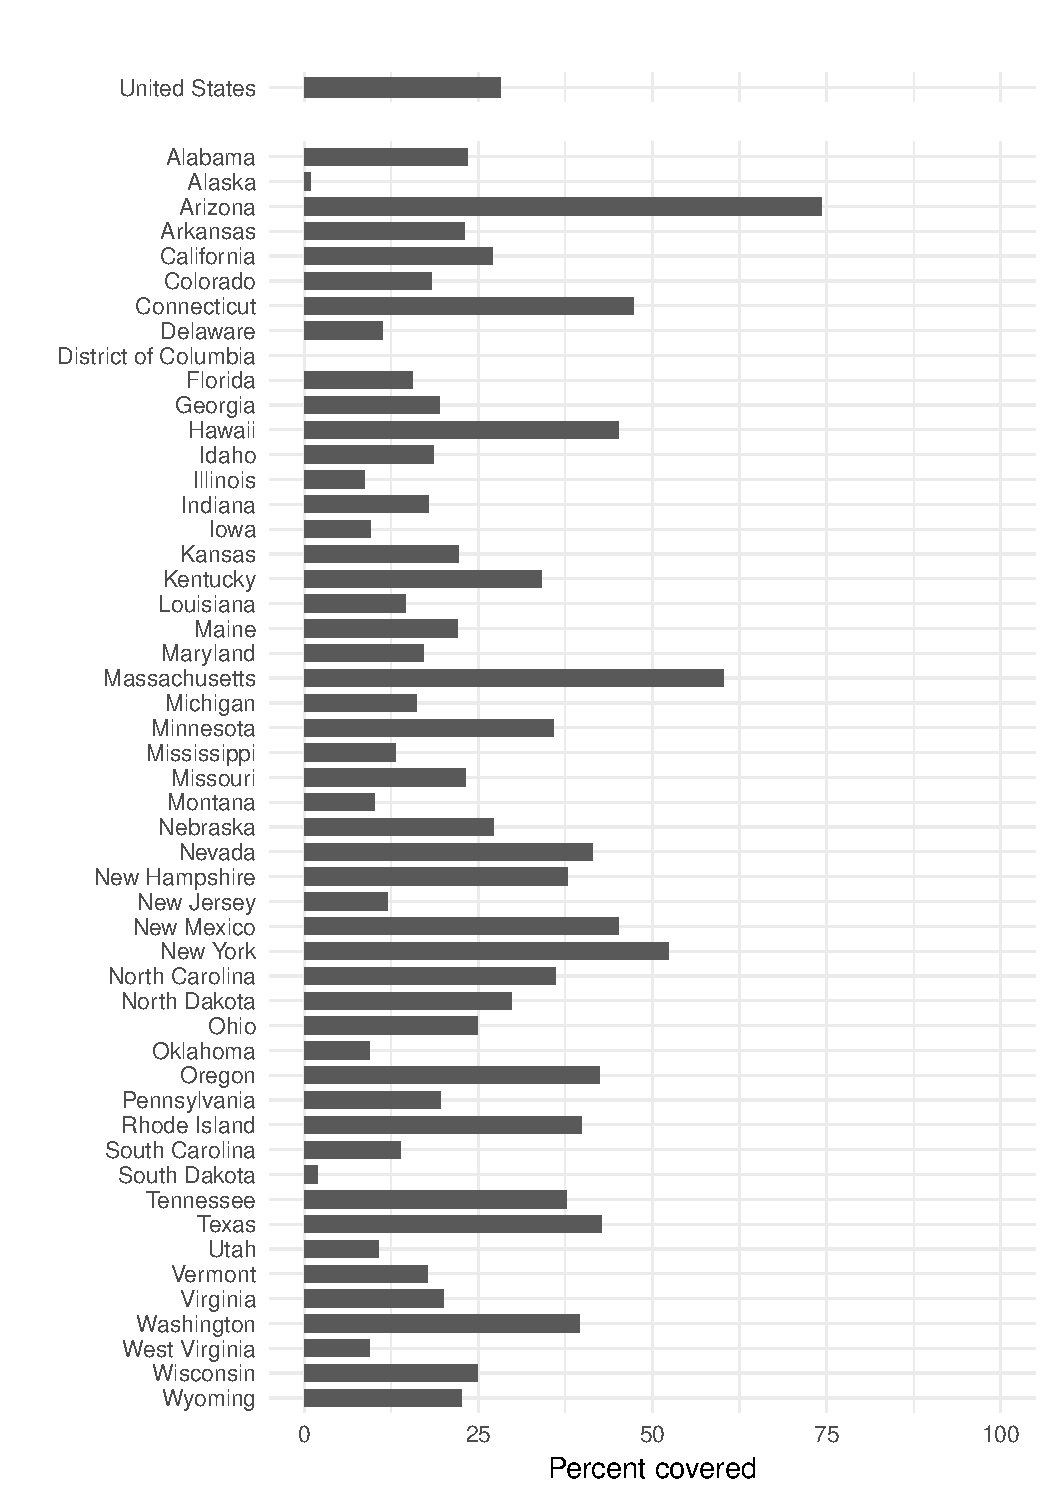
\includegraphics[width=0.9\linewidth,height=0.9\textheight]{figures/coverage_states.pdf}
\end{figure}

We use the resulting list of websites to acccess their copies stored in the Internet Archive's Wayback Machine. To this end, we rely on the Ruby Gem 'Wayback Machine Downloader'\footnote{https://github.com/hartator/wayback-machine-downloader} (WbMD). We supply the URL that each .gov website redirects to to the WbMD, which then downloads every file present in the WbM from a snapshot in October 2016, or, if not available, as soon as possible after this point.

<Note: We have not actually done this last step for all websites (however, the R script which runs the Ruby package is already set up to do so once we need to). Instead 10 websites were randomly sampled from an older version of the GSA list, which still contained counties and townships, which is why one of the 10 websites is from Dutchess County, NY.>

It would be fine to focus on Indiana as a case. First, we need to answer some preliminary questions about the data.

\begin{enumerate}

\item For what percentage and number of IN cities can we find data from the WBM?
\item For how many election cycles can we find political leadership data for these matched cities?
\item In what number and percentage of cities is the local leadership majority Republican? 
\item Relatedly, in a typical election cycle, for how many cities do we see a transition in party leadership (i.e., a shift from majority D (R) to majority (R) D). 

\end{enumerate}

\begin{enumerate}
	
	\item 30 cities, with a combined population of 1,180,435. However, since only cities (as opposed to towns and villages) hold mayoral elections, only 16 of these, with a combined population of 1,094,383 can be matched to the election data.
	\item 2015, 2011, 2007, 2003.
	\item Of the 16 cities, 7 have Republican mayors after the 2015 elections.
	\item In 6 cases, a shift of party control occurs, with 4 of these being Republican --> Democratic. 
	
\end{enumerate}




\section{Running Application: Party Differences in Municipal Websites}


\begin{landscape}
\begin{table}[htbp]
	%\caption{}
	\begin{tabular}{|p{2cm}|c|p{3cm}|p{12cm}|l|}
		\hline
		Names & Year & Journal & Findings & Important? \\ \hline
		Benedictis-Kessner, Justin De
		Warshaw, Christopher & 2016 & JOP* & Regression discontinuity design. Democratic mayors spend more (but it is unclear on what, not the typical Democratic issue-areas), issue more debt, pay more interest & Yes \\ \hline
		Caughey, Devin
		Warshaw, Christopher
		Xu, Yiqing & 2015 & Working Paper & Regression discontinuity design. Partisan composition of state governments affects state policy liberalism (composite index for the areas of social welfare, taxation, labor, civil rights, women’s rights, moral legislation, family planning, environment). & Somewhat \\ \hline
		Einstein, Katherine Levine
		Kogan, Vladimir & 2015 & Urban Affairs Review & Cities with more Democratic citizens spend more; more progressive (rather than regressive) forms of taxation; pursue intergov. aid more; spend more on police, fire, parks \& recreation & Somewhat \\ \hline
		Einstein, Katherine Levine
		Glick, David M. & 2015 & Working Paper & Survey of 72 mayors. Unlike Republican mayors, roughly half of Democrats seem to agree that cities should aim to reduce inequality. Democratic mayors also seem to favor redistribution to accomplish that goal. & Somewhat \\ \hline
		Kiewiet, D Roderick
		Mccubbins, Mathew D & 2014 & Annual Review & City budgets have been severeley constrained since the Great Recession. Spending has thus decreased in general. Lack of funds means that there is not much discretion for partisanship. & Somewhat \\ \hline
		Tausanovitch, Chris
		Warshaw, Christopher & 2014 & APSR* & Cities are responsive (taxes, expenditures, regressiveness of taxation) to citizens' conservatism/liberalism. Partisan elections do not make cities more or less responsive. & Yes \\ \hline
		Guillamón, Ma Dolores
		Bastida, Francisco
		Benito, Bernardino & 2013 & European Journal of Law and Economics & Police spending in Spain. Conservative parties spend more on police. Spending is higher before elections. Also contains a useful overview of the literature. & Yes \\ \hline
	\end{tabular}
	\label{}
\end{table}
\end{landscape}

\begin{landscape}
	\begin{table}[htbp]
		%\caption{}
		\begin{tabular}{|p{2cm}|c|p{3cm}|p{12cm}|l|}
			\hline
			Names & Year & Journal & Findings & Important? \\ \hline
			Gerber, Elisabeth R. & 2013 & Cityscape & Partisanship of both citizens and elected city officials separately affect climate policy. & Yes \\ \hline
			Solé-Ollé, Albert
			Viladecans-Marsal, Elisabet & 2013 & Journal of Urban Economics & Spanish cities. The authors "employ a regression discontinuity design to document that cities controlled by left-wing parties convert much less land from rural to urban uses than is the case in similar cities con- trolled by the right". Partisanship might also affect housing construction and price growth. & Yes \\ \hline
			Gerber, Elisabeth R.
			Hopkins, Daniel J. & 2011 & AJPS & Regression discontinuity design. Democratic mayors spend less on public safety. All other policy areas (including taxation) are unaffected. & Yes \\ \hline
			Trounstine, Jessica & 2010 & Annual Review & Race and ethnicity in local elections (not relevant to us). Partisan elections have higher turnout; non-partisan elections still tend to have some partisanship in them because voters learn about party of candidates from media. Non-partisan elections favor Republicans/upper class. Mixed evidence for whether partisanship of mayor is important for policy. & Somewhat \\ \hline
			Palus, Christine Kelleher & 2010 & State and Local Government Review & Ideology (liberal/conservative) of citizen is well represented by gov. spending in five areas: (1) community development, housing, and conservation, (2) health and human services, (3) culture, the arts, and recreation, (4) environmental programs, and (5) transportation. & Somewhat \\ \hline
			Ferreira, Fernando
			Gyourko, Joseph & 2009 & The Quarterly Journal of Economics & Regression discontinuity design. Null results for spending and city gov. size with regard to mayor partisanship. & Yes \\ \hline
			Ansolabehere, Stephen
			Snyder, James M. & 2006 & Scandinavian Journal of Economics & Despite the journal, this is about the U.S. The important finding (for us) is the fact that counties whose government is controlled by the same party as the state government, receive more funding (county's share of state transfers, normalized by county pop.) from the state. & Somewhat \\ \hline
			Murphy, Russell D. & 2002 & Annual Review & Not useful. Too philosophical; mostly cites papers written a hundred years ago. Also exclusively about larger cities. & No \\ \hline
		\end{tabular}
		\label{}
	\end{table}
\end{landscape}

\begin{landscape}
	\begin{table}[htbp]
		%\caption{}
		\begin{tabular}{|p{2cm}|c|p{3cm}|p{12cm}|l|}
			\hline
			Names & Year & Journal & Findings & Important? \\ \hline
			Armstrong, Cory L. & 2011 & Government Information Quarterly & Comparison of county and school board websites in Florida (where the two align) with regard to transparency (presence or absence of public records). Manual content analysis (undergrads told to look around for 15 minutes). School board websites, more professional websites, and websites in Republican-dominated counties are found to be more transparent. & Yes \\ \hline
			Cegarra-Navarro, Juan
			Pachón, José
			Cegarra, José & 2012 & International Journal of Information Management & Survey of Spanish municipal government officials (specifically, the city website managers). Respondents are asked about the features of their websites, the level of civic engagement and the size of their municipality. More sophisticated websites are correlated with greater civic engagement and greater use of e-government functions. & Yes \\ \hline
			Dolson, Jordan
			Young, Robert & 2012 & Canadian Journal of Urban Research & Determinants of website content. Three categories: e-content (city information on website), e-participation, social media use. Tables on page 15 show frequencies of these categories across sites, and might be useful to inform our topics. Larger cities have better websites. Population growth and immigration are also tested, but the findings are somewhat inconclusive. & Yes \\ \hline
			Feeney, Mary K.
			Brown, Adrian & 2017 & Government Information Quarterly & 500 U.S. city websites at two points in time (2010-2014). Count model of website features regarding information, e-services, utilities, transparency and civic engagement. Having a larger population leads to more features. Relying on a website contractor leads to more information and transparency. The authors say that mayor-councils are negatively correlated with website sophistication, but their regression tables state the opposite. & Yes \\ \hline
			Kaylor, Charles
			Deshazo, Randy
			Van Eck, David & 2001 & Government Information Quarterly & Model of best practices of e-government. Table 1 lists a number of possible ways this manifests, could be useful for our theory. & Somewhat \\ \hline
			Ansolabehere, Stephen
			Urban, Florian & 2002 & Cities & Websites of 20 major cities across the world. Is website content correlated with city characteristics? Not particularly systematic, and the findings are inconclusive. & Somewhat \\ \hline
			Jeffres, Leo W.
			Lin, Carolyn A. & 2006 & Journal of Computer-Mediated Communication & 50 largest metropolitan areas in the U.S. Features include information about city, opportunities for citizen feedback, galleries of photos, links, etc.  Purely descriptive analysis, doesn't contain anything that isn't covered in any of the other aricles. & No \\ \hline
		\end{tabular}
		\label{}
	\end{table}
\end{landscape}










